\documentclass{article}


\usepackage[utf8]{inputenc}
\usepackage[a4paper, total={6in, 9in}]{geometry}
\usepackage{braket}
\usepackage{xcolor}
\usepackage{amsmath}
\usepackage{amsfonts}
\usepackage{tikz}
\usepackage{svg}
\usepackage{graphicx}
\usepackage{media9}
\usepackage{float}
\usetikzlibrary{calc}
\usepackage{array}
\usepackage[ruled,vlined,linesnumbered]{algorithm2e}

\usepackage[
backend=biber,
style=alphabetic,
sorting=ynt
]{biblatex}



\newcommand{\commentt}[1]{\textcolor{blue}{ \textbf{[COMMENT]} #1}}
\newcommand{\ctt}[1]{\commentt{#1}}
\newcommand{\prb}[1]{ \mathbf{Pr} \left[ {#1} \right]}
\newcommand{\onotation}[1]{\(\mathcal{O} \left( {#1}  \right) \)}
\newcommand{\ona}[1]{\onotation{#1}}
\newcommand{\nvar}[2]{ \( #1_{1}, #1_{2} ... #1_{#2}  \) }
%\newenvironment{proof}[0]{\paragraph{Proof.}}{}
%\newenvironment{remark}[0]{\textit{remark}}{}
\newenvironment{cor}[0]{\paragraph{Corollary.}}{}
\newenvironment{example}[0]{\paragraph{Example.}}{}
%\newenvironment{thm}[0]{\paragraph{Theorem.}}{}
\newtheorem{prop}{Proposition}
\newtheorem{ex}{Exercise}
\newtheorem{sol}{Solution}
\newtheorem{theorem}{Theorem} 		
\newtheorem{thm}{Theorem}[section]
\newtheorem{conj}[thm]{Conjecture} 	
\newtheorem{lemma}[thm]{Lemma}
\newtheorem{corollary}[thm]{Corollary} 
\newtheorem{claim}[thm]{Claim}
\newtheorem{proposition}[thm]{Proposition}
\newtheorem{definition}{Definition} 
\newtheorem{remark}{Remark}
 


% \addbibresource{sample.bib} %Import the bibliography file
\begin{document}    
\maketitle
\newcommand*{\RECITATION}{}%

\begin{document}
\chapter{Introduction to Algorithms.}
%, Correctness and Efficiency
\ifdefined\RECITATION
\else
Computer science differs from other scientific disciplines in that it focuses not on solving or making discoveries, but on questioning how good is our current understanding. The fact that one has successfully come up with an idea for a certain problem immediately raises the question of optimality. At the most basic level, we would like to answer what is the 'best' \marginnote[Note 1: text for left-hand side text]{Note 1: text for right-hand side of pages, it is set justified.} program that exists for a particular problem. To do so, we must have a notation that allows us to determine if an algorithm is indeed solving the task, quantify its performance, and compare it to other algorithms. In this chapter, we introduce this basic notation. The chapter is divided into two main parts: the first is about induction, a mathematical technique for proving claims, and the second presents asymptotic notation, which we use to describe the behavior of algorithms over large inputs.
\fi
\section{Peaks-Finding.}
\begin{example}[Leading Example.]
Consider an \(n\)-length array $A$ such that~$A_1,A_2,....,A_n~\in~\mathbb{R}$. We will say that $A_{j}$ is a peak (local minimum) if he's greater than his neighbors. Namely, $A_{i} \ge A_{i\pm1}$ if $i\pm 1 \in [n]$. Whenever $i\pm 1$ is not in the range $[n]$, we will define the inequality $A_{i} \ge A_{i\pm 1}$ to hold trivially. For example, for $n=1$, $A_{1}=A_{n}$ is always a peak. Write an algorithm that, given $A$, returns the position of an arbitrary peak.
\end{example}


\begin{example}{Warming up.} \label{example:func} How many peaks do the following arrays contain?
  \begin{enumerate}
    \item $A[i] = 1$   $\forall i \in [n]$
    \item $A[i] = \begin{cases}
        i & i < n/2 \\
        n/2 - i & \text{else}
      \end{cases}$
    \item $A[i] = i $  $\forall i \in [n]$
  \end{enumerate}
\end{example}

\section{Naive solution.}
To better understand the problem, let's first examine a simple solution before proposing a more intriguing one. Consider the algorithm examining each of the items $A_{i}$ one by one.
\begin{algorithm}
\KwResult{returns a peak of \(A_1 ... A_n \in \mathbb{R}^n \)  }
\caption{naive peak-find alg.}
 \For{ \(i \in [n] \) } { 
   \If { $A_{i}$ is a peak }{
        \Return $i$
        }
    } 
\end{algorithm}
\paragraph{Correctness.}
We will say that an algorithm is correct, with respect to a given task, if it computes the task for any input. Let's prove that the above algorithm is doing the job. 

\begin{proof}
%  Assume towards contradiction that there exists an $n$-length array $A$ such that the algorithm peak-find fails to find one of its peaks, in particular, the Alg. either returns $j^{\prime}\in [n]$ such that $A_{j^{\prime}}$ is not a peak or not return at all (never reach line (3)). Let's handle first the case in which retruning indeed occurred. Denote by $j$ the first position of a peak in $A$, and note that if the algorithm gets to line (2) in the $j$th iteration then either it returns $j$ or $A_{j}$ is not a peak.
%  Hence it must hold that $j^{\prime} < j$. But a satisfaction of the condition on line (2) can happen only if $A_{j^{\prime}}$ is a peak, which contradicts the minimality of $j$.
%
%  In the case that no position has been returned, In particular the algorithm didn't return in any of the first $j$ iterations and get's in to iteration number $j+1$, which means that the conidition on line (2) was not satisfied in contradiction to the fact that $A_{j}$ is a peak. 
%
Assume towards contradiction that there exists an $n$-length array $A$ such that the algorithm peak-find fails to find one of its peaks, in particular, the Alg. either returns $j^{\prime}\in [n]$ such that $A_{j^{\prime}}$ is not a peak or does not return at all (never reach line (3)). Let's handle first the case in which returning indeed occurred. Denote by $j$ the first position of a peak in $A$, and note that if the algorithm gets to line (2) in the $j$th iteration then either it returns $j$ or $A_{j}$ is not a peak.
  Hence it must hold that $j^{\prime} < j$. But satisfaction of the condition on line (2) can happen only if $A_{j^{\prime}}$ is a peak, which contradicts the minimality of $j$. In the case that no position has been returned, it follows that the algorithm didn't return in any of the first $j$ iterations and gets to iteration number $j+1$, which means that the condition on line (2) was not satisfied in contradiction to the fact that $A_{j}$ is a peak.
\end{proof}

\paragraph{Running Time.} 
Question, How would you compare the performance of two different algorithms? What will be the running time of the naive peak-find algorithm? On the lecture you will see a well-defined way to treat such questions, but for the sake of getting the general picture, let's assume that we pay for any comparison a quanta of processing time, and in overall, checking if an item in a given position is a peak, cost at most $c\in \mathbb{N}$ time, a constant independent on $n$.

Question, In the worst case scenario, how many local checks does peak-finding do? For the third example in~\Cref{example:func}, the naive algorithm will have to check each item, so the running time adds up to at most $c \cdot n$.

\section{Naive alg. recursive version.}
Now, we will show a recursive version of the navie peak-find algorithm for demonstrating how correctness can be proved by induction. 
\begin{algorithm}
\KwResult{returns a peak of \(A_1 ... A_n \in \mathbb{R}^n \)  }
\caption{naive recursive peak-find alg.}
 \If { $A_{1} \ge A[2]$ or $n=1$ }{
   \Return 1
 }
 \Return 1 + peak-find$(A_{2}, .. A_{n})$
 \end{algorithm}

 \begin{claim} \label{claim:subarray} 
Let $A = A_1, \dots, A_n$ be an array, and $A' = A_2, A_3, \dots, A_n$ be the $n-1$ length array obtained by taking all of $A$'s items except the first. If $A_1 \le A_2$, then any peak of $A'$ is also a peak of $A$.
\end{claim}
\begin{proof} 
Let $A^{\prime}_{j}$ be a peak of $A^{\prime}$. Split into cases upon on the value of $j$. If $n-1 > j > 1$, then $A^{\prime}_{j} \ge A^{\prime}_{j \pm 1}$, but for any $j \in [2, n-2]$ we have $A^{\prime}_{j} = A_{j+1}$ and therefore $A_{j+1} \ge A_{j+1 \pm 1} \Rightarrow A_{j+1}$ is a peak in $A$. If $j^{\prime} = 1$, then $A^{\prime}_{1} > A^{\prime}_{2} \Rightarrow A_{2} \ge A_{3}$ and by combining the assumption that $A_{1} \le A_{2}$ we have that $A_{2} \ge A_{1}, A_{3}$. So $A_{2} = A^{\prime}_{1}$ is also a peak. The last case $j = n-1$ is left as an exercise.
\end{proof}

One can prove a much more general claim by following almost the same argument presented above.

 \begin{claim} \label{claim:subarraymiddle} 
   Let $A = A_1, \dots, A_n$ be an array, and $A' = A_{j+1}, A_{j+2}, \dots, A_n$ be the $n-j$ length array. If $A_j \le A_{j+1}$, then any peak of $A'$ is also a peak of $A$.
\end{claim}
\section{Induction. (Might not appear in the recitation.)} 
\ifdefined\RECITATION
\else
Suppose that a teacher, who is standing in front of his class, is willing to prove that he can reach the door at the corner. One obvious way to do so is to actually reach the door; that is, move physically to it and declare success. For small classes containing a small number of students, this protocol might even be efficient, lasting less than several seconds. But what if the class is really big, maybe the length and width of a football stadium? In that case, proving by doing might take time. So the obvious question to ask is, what else can we do? Is there a more efficient way to prove this?

Indeed, there is. Instead of proving that he can reach the door, he can prove that while he do not stand next to the door, nothing can stop him from keeping moving forward. If that is indeed the case, then it's clear that not reaching the door in the end would be a contradiction to being just one step away from it (why?), which, in turn, would also contradict being two steps away from it. Repeating this argument leads to a contradiction for the fact that the teacher was in the classroom at the beginning.
\fi
\paragraph{What is induction?}~\begin{enumerate}
    \item A mathematical proof technique. It is essentially used to prove that a property \(P(n)\) holds for every natural number \(n\).
    \item The method of induction requires two cases to be proved:
    \begin{enumerate}
        \item The first case, called the base case, proves that the property holds for the first element.
        \item The second case, called the induction step, proves that if the property holds for one natural number, then it holds for the next natural number.
    \end{enumerate}
    \item The domino metaphor. 
\end{enumerate}
\paragraph{The two types of induction, their steps, and why it makes sense} (Strong vs Weak) - Emphasize the change in the induction step.
\begin{example}[Weak induction] Prove that $ \forall n \in  \mathbb{N}$,$\sum_{i=0}^{n}{i} = \frac{n(n+1)}{2}$.
\begin{proof} Base: For \(n = 1\), \(\sum_{i=0}^{1}{1} = 1 = \frac{(1+1)\cdot 1}{2} \). Assumption: Assume that the claim holds for \(n\).Step: 
\begin{equation*}
  \begin{split}
 \sum_{i=0}^{n+1}{i} = & \left( \sum_{i=0}^{n}{i} \right) + n+1 = \frac{n(n+1)}{2} + n + 1 \\
 = & \frac{n(n+1) + 2\cdot (n+1)}{2} = \frac{(n+1)(n+2)}{2} 
  \end{split}
\end{equation*}
\end{proof}
\end{example}
\begin{example}[Weak induction.] Let \(q\in \mathbb{R} / \{1\}\), consider the geometric series \( 1,q,q^2,q^3....q^k...\). Prove that the sum of the first \(k\) elements is \begin{equation*}
     1+q+q^2+...+q^{k-1}+q^k = \frac{q^{k+1}-1}{q-1}
\end{equation*}

\begin{proof} Base: For \(n = 1\), we get \( \frac{q^{k+1}-1}{q-1} = \frac{q-1}{q-1} = 1\). 
Assumption: Assume that the claim holds for \(k\). then:
Step: 
\begin{equation*}
\begin{split}
    1+q+q^2+...+q^{k-1}+q^k + q^{k+1} &=  \frac{q^{k}-1}{q-1} + q^{k+1}  = \frac{q^{k+1}-1 +q^{k+1}\left(q-1\right) }{q-1} = \\ &\frac{\textcolor{red}{q^{k+1}}-1 +q^{k+2} - \textcolor{red}{q^{k+1}}  }{q-1} = \frac{q^{k+2}-1}{q-1} 
\end{split}
\end{equation*}
\end{proof}
\end{example}
% \ctt{Finish the induction proof and add alternative proof by counting. I am not sure what is favored, exposing both ways (at the first example) will make clear that induction is only a single proofing tool and surly not the only one. Yet from didactic point of view, it might confuses. }

\begin{example}[Strong induction] 
  Let there be a chocolate bar that consists of \(n\) square chocolate blocks. Then it takes exactly \(n - 1\) snaps to separate it into the \(n\) squares no matter how we split it.

  \begin{proof} By strong induction. Base: For \(n = 1\), it is clear that we need \(0\) snaps. Assumption: Assume that for \textbf{every} \(m < n \), this claim holds.


Step: We have in our hand the given chocolate bar with \(n\) square chocolate blocks. Then we may snap it anywhere we like, to get two new chocolate bars: one with some \( k \in [n]\) chocolate blocks and one with \(n - k\) chocolate blocks. From the induction assumption, we know that it takes \(k - 1\) snaps to separate the first bar, and \(n - k - 1\) snaps for the second one. And to sum them up, we got exactly \[ (k - 1) + (n - k - 1) + 1 = n - 1 \] snaps.
\end{proof}
\end{example}

We are ready to prove the correcntess of the recursive version by induction using \Cref{claim:subarray}. 

\begin{enumerate}
  \item Base, single element array. Trivial. 
  \item Assumption, Assume that for any $m$-length array, such that $m<n$ the alg returns a peak. 
  \item Step, consider an array $A$ of length $n$. If $A_1$ is a peak, then the algorithm answers affirmatively on the first check, returning $1$ and we are done. If not, namely $A_1 < A_2$, then by using \Cref{claim:subarray} we have that any peak of $A' = A_2, A_3, \dots, A_n$ is also a peak of $A$. The length of $A'$ is $n-1 < n$. Thus, by the induction assumption, the algorithm succeeds in returning on $A'$ a peak which is also a peak of $A$.
\end{enumerate}

\section{An attempt for sophisticated solution.}
We saw that we can find an arbitrary peak at $c\cdot n$ time, which raises the question, can we do better? Do we really have to touch all the elements to find a local maxima? Next, we will see two attempts to catch a peak at logarithmic cost. The first attempt fails to achieve correctness, but analyzing exactly why will guide us on how to come up with both an efficient and correct algorithm.
\begin{algorithm}
\KwResult{returns a peak of \(A_1 ... A_n \in \mathbb{R}^n \)  }
\caption{fail attempt for more sophisticated alg. }
        $ i \leftarrow  \lceil n/2 \rceil $\\
        \If { $A_{i}$ is a peak }{
          \Return $i$
        }
        \Else { 
          \Return $i - 1  + $ find-peak$\left(A_{i},A_{i+1}..A_{n}\right)$
        }
\end{algorithm}

Let's try to 'prove' it.  
\begin{enumerate}
 \item Base, single element array. Trivial. 
  \item Assumption, Assume that for any $m$-length array, such that $m<n$ the alg returns a peak. 
  \item Step. If $A_{n/2}$ is a peak, we're done. What happens if it isn't? Is it still true that any peak of $A_{i},A_{i+1}, \ldots, A_{n}$ is also a peak of $A$? Consider, for example, $A[i] = n - i$.
\end{enumerate}

\section{Sophisticated solution.}
The example above points to the fact that we would like to have a similar claim to \Cref{claim:subarraymiddle} that relates the peaks of the split array to the original one.  
\begin{algorithm}
\KwResult{returns a peak of \(A_1 ... A_n \in \mathbb{R}^n \)  }
\caption{sophisticated alg.}
$ i \leftarrow  \lceil n/2 \rceil $\\
        \If { $A_{i}$ is a peak }{
          \Return $i$
        }
        \ElseIf { $A_{i-1} \le A_{i}$ } { 
          \Return $i + $ find-peak$\left(A_{i+1}..A_{n}\right)$
        }
        \Else { 
          \Return find-peak$\left(A_{1},A_{2},A_{3}..A_{i-1}\right)$
        }
\end{algorithm}
Let's prove correction by induction.
\begin{proof}
\begin{enumerate}
  \item Base, single element array. Trivial. 
  \item Assumption, Assume that for any $m$-length array, such that $m<n$ the alg returns a peak. 
  \item Step, Consider an array $A$ of length $n$. If $A_{\lceil n/2 \rceil}$ is a peak, then the algorithm answers affirmatively on the first check, returning $\lceil n/2 \rceil$ and we are done. If not, then either $A_{\lceil n/2 \rceil} < A_{\lceil n/2 \rceil - 1}$ or $A_{\lceil n/2 \rceil} < A_{\lceil n/2 \rceil + 1}$. We have already handled the first case, that is, using \Cref{claim:subarraymiddle} we have that any peak of $A' = A_{\lceil n/2 \rceil + 1}, A_{\lceil n/2 \rceil + 2}, \dots, A_n$ is also a peak of $A$. The length of $A'$ is $n/2 < n$. So by the induction assumption, in the case where $A_{\lceil n/2 \rceil} < A_{\lceil n/2 \rceil - 1}$ the algorithm returns a peak. In the other case, we have $A_{\lceil n/2 \rceil} < A_{\lceil n/2 \rceil + 1}$ (otherwise $A_{\lceil n/2 \rceil}$ would be a peak). We leave finishing the proof as an exercise.
\end{enumerate}

\end{proof}

\ctt{  
  In the previous version of the recitation, the first recursive call was to find-peak$\left(A_{i},A_{i+1}..A_{n}\right)$. However, in the case where $n=2$, we have that $A_{i}=A_1$, so it does not hold that $|A^{\prime}| < |A|$. And we cann't use the induction assumption. 
}


What's the running time? Denote by $T\left( n \right)$ an upper bound on the running time. We claim that $T(n) \le c \log (n) + c$, let's prove it by induction.
\begin{proof}
     
\begin{enumerate}
  \item Base. For the base case, $n=1$ we get that $c \log(1) + c =  c$ on the other hand only a single check made by the algorithm, so indeed the base case holds.
  \item Induction Assumption. Assume that for any $m < n$, the algorithm runs in at most $c \log(m) + c$ time.
  \item Step. Notice that in the worst case, $\lceil n/2 \rceil$ is not a peak, and the algorithm calls itself recursively immediately after paying $c$ in the first check. Hence: \begin{equation*}
      \begin{split}    
    T\left(n\right) & \le c + T\left(n/2\right) \le c + c \log\left( \lceil n/2 \rceil \right) + c\\
  & = c \log (2) +  c \log\left( \lceil n/2 \rceil  \right) + c = c \log\left(2 \left(\lceil n/2 \rceil \right) \right) + c\\
  & \le c \log \left( n  \right)    
      \end{split}
    \end{equation*}
\end{enumerate}
\end{proof}




% \section{Time Planning.}
% \begin{enumerate}
%     \item Welcome words, general information, listing the recitation topics \& QA. 7\textbf{m} (section 1).
%     \item Explain (remind) induction and presenting the first first example. 10\textbf{m}.
%     \item Second weak induction example 4\textbf{m}.
%     \item Strong induction 7\textbf{m}.
%     \item Introduce, the big O. explain the object shortly, plot graphs. yet still not formal definitions. 7\textbf{m}.  
%     \item Shoot the definitions of the \(O, \Omega, \Theta\) at one. 7\textbf{m}.
%     \item 3\textbf{m} spare + break. 
%     \item Review again the asymptotic notations, with examples from section 4. Q\&A. 7\textbf{m}
%     \item Lemma 21 7\textbf{m}
%     \item Claim 22 7\textbf{m}
%     \item The claim beneath Claim 22 7\textbf{m}
%     \item Example 23 7\textbf{m} (should take more time, the above claims will pay the tax). 
%     \item Logarithmic Rules 7\textbf{m}. 
% \end{enumerate}
% \section{General Course Information.}
% \begin{enumerate}
%     \item Introduce yourself
%     \item course mail: huji.dast.2022a@gmail.com
%     \item targilim scoring: 0.85 \( \cdot \) Test + 0.15 \( \cdot \) Average(\(N - 2\)). 
% \item  introduction to the course: \begin{enumerate}
%     \item  It’s important \& fun: \begin{enumerate}
%         \item We going to learn some data structures: Heaps, Trees, Hash Tables
%         \item And some algorithms: Sorting, Minimal Spanning Tree, Shortest Path
%     \end{enumerate}
%     \item Doing your homework by yourself is the best way to improve your solving problems skill.
% \end{enumerate}
% \end{enumerate}

% \paragraph{Abstract.} Today we will cover induction, infinite series, and asymptotic notation. These tools will come in handy (in the next couple of weeks) when we want to find the runtime complexity of an algorithm, specifically using the ’Master Theorem’, to give asymptotic bounds for recursion relations, and to prove loop invariants using (finite) induction.


\newpage
%\documentclass{article}


\usepackage[utf8]{inputenc}
\usepackage[a4paper, total={6in, 9in}]{geometry}
\usepackage{braket}
\usepackage{xcolor}
\usepackage{amsmath}
\usepackage{amsfonts}
\usepackage{tikz}
\usepackage{svg}
\usepackage{graphicx}
\usepackage{media9}
\usepackage{float}
\usetikzlibrary{calc}
\usepackage{array}
\usepackage[ruled,vlined,linesnumbered]{algorithm2e}

\usepackage[
backend=biber,
style=alphabetic,
sorting=ynt
]{biblatex}



\newcommand{\commentt}[1]{\textcolor{blue}{ \textbf{[COMMENT]} #1}}
\newcommand{\ctt}[1]{\commentt{#1}}
\newcommand{\prb}[1]{ \mathbf{Pr} \left[ {#1} \right]}
\newcommand{\onotation}[1]{\(\mathcal{O} \left( {#1}  \right) \)}
\newcommand{\ona}[1]{\onotation{#1}}
\newcommand{\nvar}[2]{ \( #1_{1}, #1_{2} ... #1_{#2}  \) }
%\newenvironment{proof}[0]{\paragraph{Proof.}}{}
%\newenvironment{remark}[0]{\textit{remark}}{}
\newenvironment{cor}[0]{\paragraph{Corollary.}}{}
\newenvironment{example}[0]{\paragraph{Example.}}{}
%\newenvironment{thm}[0]{\paragraph{Theorem.}}{}
\newtheorem{prop}{Proposition}
\newtheorem{ex}{Exercise}
\newtheorem{sol}{Solution}
\newtheorem{theorem}{Theorem} 		
\newtheorem{thm}{Theorem}[section]
\newtheorem{conj}[thm]{Conjecture} 	
\newtheorem{lemma}[thm]{Lemma}
\newtheorem{corollary}[thm]{Corollary} 
\newtheorem{claim}[thm]{Claim}
\newtheorem{proposition}[thm]{Proposition}
\newtheorem{definition}{Definition} 
\newtheorem{remark}{Remark}
 


% \addbibresource{sample.bib} %Import the bibliography file
\begin{document}    
\maketitle
    
\chapter{Correctness - Recitation 2} 
%\author{Correctness proofs and computational complexity. }
%\makechapter 
%\begin{paragraph}
    Proving algorithms correctness is necessary to guarantee that our code computes its goal for every given input. In that recitation, we will examine several algorithms, analyze theirs running time and memory consumption, and prove they are correct.   
%\end{paragraph}


\begin{example}[Leading Example.]
Consider \(n\) numbers \(a_1,a_2,....,a_n \in \mathbb{R}\). Given set \(Q\) of \(|Q|\) queries, such each query \(q \in Q\) is a tuple \( (i,j) \in [n] \times [n] \). Write an algorithm that calculates the \(\max_{i\le k\le j}{a_k} \). 
\end{example}
\section{Correctness And Loop Invariant.}

\paragraph{Correctness.} We will say that an algorithm \( \mathcal{A}\) (an ordered set of operations) computes \( f:D_1 \rightarrow D_2 \) if for every \(x \in D_1\) the following equality holds \(f(x) = \mathcal{A}(x)\). Sometimes when it's obvious what is the goal function \(f\), we will abbreviate and say that \( \mathcal{A}\) is correct.       

Examples of functions \(f\) might be: file saving, summing numbers, or posting a message in the forum.  

\paragraph{Loop Invariant.} Loop Invariant \marginpar[Note 1: text for left-hand side text]{Note 1: text for right-hand side of pages, it is set justified.}is a property that characteristic a loop segment code  and satisfy the following conditions: 
\begin{enumerate}
    \item Initialization. The property holds (even) before the first iteration of the loop.   
    \item Conservation. As long as one performs the loop iterations, the property still holds.
    \item (optional) Termination. Exiting from the loop carrying information.
\end{enumerate}

\begin{example} Before dealing with the hard problem, let us face the naive algorithm to find the maximum of a given array.

\begin{algorithm}
\KwResult{returns the maximum of \(a_1 ... a_n \in \mathbb{R}^n \)  }
\caption{naive maximum alg.}
\Fn{max( $a_{1} .. a_{n}$ )}{
 \For{ \(i \in [n] \) } { 
        \( j \leftarrow 1 \) \\
        \ \\
        \While{ \(j \le [n] \) and \( a_i \ge a_j \) } {
        \( j \leftarrow j + 1 \)    
        }
        \\
        \ \\ 
        \If { \(j = n+1\) }{
        \Return \(a_i\)
        }
    } 
\Return \( \Delta \) \\  
}
\end{algorithm}

\begin{claim} Consider the while loop. The property: \textit{"for every \(j^\prime < j \le n+1 \Rightarrow a_{j^\prime} \le a_i \)"} is a loop invariant that is associated with it. 
\end{claim}
\begin{proof} first, the initialization condition holds, as the at the first iteration \(j=1\) and therefore the property is trivial.
Assume by induction, that for every \(m < j\) the property is correct, and consider the \(j\)-th iteration. If back again to line (5), then it means that \( (j-1) < n\) and \( a_{j-1} \le a_{i} \). Combining the above with the induction assumption yields that \(a_i \ge a_{j-1},a_{j-2}, ... a_{1}\).    
\end{proof}

\paragraph{Correctness Proof.} Split into cases, First if the algorithm return result at line (9), then due to the loop invariant, combining the fact that \( j = n + 1\), it holds that for every \(j^\prime  \le n < j \Rightarrow a_i \ge a_{j^\prime} \)  i.e \(a_i\) is the maximum of \(a_1, .... a_n \). The second case, in which the algorithm returns \( \Delta \) at line number (10) contradicts the fact that \(n\) is finite, and left as an exercise.  the running time is \( O(n^2) \) and the space consumption is \(O(n)\). 

\paragraph{Loop Invariant In The Cleverer Alg.} Consider now the linear time algorithm:

\begin{algorithm}[H]
% \SetAlgoLined
\KwResult{returns the maximum of \(a_1 ... a_n \in \mathbb{R}^n \)  }
\Fn{max( $a_{i} .. a_{j}$) }{
 \ \\ 
 let \(b \leftarrow a_1 \) \\ 
 \ \\ 
 \For{\(i \in [2, n] \) } { 
        \(b \leftarrow \max \left(b, a_i \right) \)
    } 
 return \( b \) 
 }
 \caption{maximum alg.}
\end{algorithm}

What is the Loop Invariant here? \textit{"at the \(i\)-th iteration, \(b = \max{ \{ a_1 ... a_{i-1} \} } \)"}. The proof is almost identical to the naive case.   
\end{example}
\section{Non-Linear Space Complexity Algorithms. }
\paragraph{Sub-Array Maximum.} Consider the leading example; It's easy to write an algorithm that answers the queries at a total time of a \( O\left( |Q| \cdot n \right) \) by answers separately on each query. Can we achieve a better upper bound?



%
\begin{algorithm}
  \caption{Sub-Array. \(O(n^2)\) space alg.}
% \SetAlgoLined
\KwResult{print the \( \max{\{ a_i ... a_j \} }\) for each query \((i,j) \in Q \) }
\Fn{max( $a_i ... a_j$ )}{
 let \(A \leftarrow \mathbb{M}^{n\times n} \) \\ 
 \ \\ 
 \For{\(i \in [n] \) } {
    \( A_{i,i} \leftarrow a_i\)
 }
 \ \\
 \For{ \(k \in [1, n]\) }{
    \For{\(i \in [n] \) } {
        \If{ \(i+k \le n\) }{
        \(A_{i,i+k} \leftarrow \max \left(A_{i,i+k-1}, a_{i+k} \right) \)
        }
    } 
}
\ \\
\For { \( q \in Q \) }{
    \(i,j \leftarrow q \) \\
    print \( A_{i,j}\)
}
}
\end{algorithm}
%

\paragraph{Claim.} Consider the outer loop at the \(k\)-th step. The following is a loop invariant: \[for \ every \ k^\prime < k ,\ s.t \ i + k^\prime \le n \Rightarrow A_{i,i+k^\prime} = \max{ \{ a_{i}, a_{i+1}, ... ,a_{i + k^\prime} \} }\]  
\textbf{Proof.} The initialization condition trivially holds, assume by induction that \( A_{i,i+k-1} = \max{\{a_i ... a_{i+k-1}\}}\) at beginning of \( k \) iteration. By the fact that \( \max(x,y,z)= \max(\max(x,y),z) \) we get that
\begin{equation*}
\begin{split}
 \max{\{a_1 ... a_{i + k-1}, a_{i+ k} \}} = \max{\{ \max{ \{ a_1 ... a_{i + k-1} \} }, a_{i+ k} \}} =  \max{\{A_{i,i+k-1}, a_{i+ k} \}}
 \end{split}    
 \end{equation*} And the right term is exactly the value which assigned to \(A_{i,i+k}\) in the end of the\(k\)-th iteration. Thus in the beginning of \( k+1 \) iteration the property is still conserved.

\paragraph{ \(O\left(n\log n\right)\) Space Solution.} Example for \(O\left(n\log n + |Q|\log n\right)\) time and \(O\left(n\log n\right)\) space algorithm. Instead of storing the whole matrix, we store only logarithmic number of rows.   

%{}
\begin{algorithm}
% \SetAlgoLined
  \caption{Sub-Array. \(O(n \log n )\) space alg.}
\KwResult{print the \( \max{\{ a_i ... a_j \} }\) for each query \((i,j) \in Q \) }
\Fn{max( $a_i ... a_j$ )}{
 let \(A \leftarrow \mathbb{M}^{n\times \log n} \) \\ 
 \ \\
 \For{\(i \in [n] \) } {
    \( A_{i,1} \leftarrow a_i\)
 }
 \ \\
 \For{ \(k \in [2,4,..,2^m,...,n]\) }{
    \For{\(i \in [n] \) } {
        \If{ \(i+k \le n\) }{
        \(A_{i,k} \leftarrow \max \left(A_{i,\frac{k}{2}},A_{i+\frac{k}{2}, \frac{k}{2}} \right) \)
        }
    } 
}
\ \\
\For { \( q \in Q \) }{
    \(i,j \leftarrow q \) \\
    decompose \(j - i \) into binary representation \(2^{t_1} + 2^{t_2} + .. +2^{t_l}\) \\
    print \( \max { \{ A_{i,2^{t_1}},A_{i+ 2^{t_1}, 2^{t_2} }, ... , A_{i+ 2^{t_1} + 2^{t_2} +.. 2^{t_{l-1}}, 2^{t_l}} \} }\)
}
}
\end{algorithm}
%



\newpage

\setcounter{chapter}{2}
\chapter{Recursive Analysis.} 
%\author{Master theorem and recursive trees.}
% 
%\begin{paragraph}
%    One of the standard methods to analyze the running time of algorithms is to express recursively the number of operations that are made. In the following recitation, we will review the techniques to handle such formulation (solve or bound).  
%\end{paragraph}
%

\section{Bounding recursive functions by hands.} Our primary tool to handle recursive relation is the Master Theorem, which was proved in the lecture. As we would like to have a more solid grasp, let's return on the calculation in the proof over a specific case. 
Assume that your algorithm analysis has brought the following recursive relation:
    \begin{example}\( T\left(n\right)  = \left\{ \begin{array}{rcl}
& 4T\left(\frac{n}{2}\right)+c\cdot n & \mbox{for }  n > 1  \\
& 1 & \mbox{else}  
\end{array}\right. \). Thus, the running time is given by \begin{equation*}
    \begin{split}
 & T\left(n\right)  = 4T\left(\frac{n}{2}\right)+c\cdot n=  4\cdot4T\left(\frac{n}{4}\right)+4c\cdot\frac{n}{2}+c\cdot n = ... = \\ & \overset{\text{\textcolor{red}{critical}}}{\overbrace{4^{h}T(1)}} + c\cdot n\left(1+\frac{4}{2}+\left(\frac{4}{2}\right)^{2}...+\left(\frac{4}{2}\right)^{h-1}\right) = 4^{h} + c\cdot n\cdot\frac{2^{h}-1}{2-1}
    \end{split}
\end{equation*}
We will call the number of iteration till the stopping condition the recursion height, and we will denote it by \(h\) . What should be the recursion height? \( 2^{h} = n \Rightarrow h =\log\left(n\right) \). So in total we get that the algorithm running time equals \( \Theta\left(n^2\right)\). 
\end{example}
\textbf{Question}, Why is the term \( 4^{h} T(1) \) so critical? Consider the case \(T\left(n\right) =  4T\left(\frac{n}{2}\right) + c \) .One popular mistake is to forget the final term, which yields a linear solution \( \Theta(n)\) (instead of quadric \( \Theta(n^2)\)).   

    \begin{example}\( T\left(n\right)  = \left\{ \begin{array}{rcl}
& 3T\left(\frac{n}{2}\right) + c\cdot n & \mbox{for }  n > 1  \\
& 1 & \mbox{else}  
\end{array}\right. \), and then the expanding yields: 
\begin{equation*}
    \begin{split}
        T\left(n\right) & = 3T\left(\frac{n}{2}\right) + c\cdot n = 3^2 T\left(\frac{n}{2^2}\right) + \frac{3}{2}cn + c\cdot n \\ 
        & =  \overset{\text{\textcolor{red}{critical}}}{\overbrace{3^{h}T(1)}} + cn\left(1 + \frac{3}{2} + \left(\frac{3}{2}\right)^2 + ...  + \left(\frac{3}{2}\right)^{h-1} \right) \\
        & h = \log_{2}\left(n\right) \Rightarrow T\left(n\right) = 3^{h}T(1) + c\cdot \textcolor{red}{n}\cdot \left(\left(\frac{3}{\textcolor{red}{2}}\right)^{\log_{2}{n}}\right) / \left(\frac{3}{2} - 1\right) \\ 
        & = \theta \left( 3^{\log_{2}(n)} \right) =  \theta \left( n^{\log 3} \right)  
    \end{split}
\end{equation*}
where \(n^{\log 3}  \sim n^{1.58} < n^2 \).
\end{example}


\section{Master Theorem, one Theorem to bound them all. }
As you might already notice, the same pattern has been used to bound both algorithms. The master theorem is the result of the recursive expansion. it classifies recursive functions at the form of \(T\left(n\right) = a\cdot T\left( \frac{n}{b} \right) + f\left(n\right) \), for positive function \(f : \mathbb{N} \rightarrow \mathbb{R}^{+} \).       

\begin{defbox}{Master Theorem, simple version.} First, Consider the case that \(f = n^c\). Let \( a \ge 1, b > 1\) and \( c \ge 0 \). then: 
\begin{enumerate}
    \item if \(\frac{a}{b^c} < 1 \) then \( T\left(n\right) = \Theta \left( n^c \right) \) \ \ \ \textbf{(\(f\) wins)}.
    \item if \(\frac{a}{b^c} = 1 \) then \( T\left(n\right) = \Theta \left( n^c \log_{b} \left(n\right) \right) \).
    \item if \(\frac{a}{b^c} > 1 \) then \( T\left(n\right) = \Theta \left( n^{\log_{b} \left(a\right)} \right) \) \ \ \ \textbf{(\(f\) loose)}.
  \end{enumerate}
\end{defbox}

\begin{example}  \( T\left(n\right)  =4T\left(\frac{n}{2}\right)+d\cdot n \Rightarrow
T\left(n\right) = \Theta\left(n^2\right)\) according to case (3). And \(T\left(n\right)  = 3T\left(\frac{n}{2}\right) + d\cdot n \Rightarrow T\left(n\right) = \Theta \left( n^{\log_{2}\left(3\right)}\right)\)
also due to case (3).
\end{example}
\begin{defbox}{Master Theorem, strong version.} 
Now, let's generalize the simple version for arbitrary positive \(f\) and let~\(a~\ge~1~,~b~>~1\). 

\newcommand{\logab}{\log_{b} \left(a\right)}

\begin{enumerate}
    \item if  \(f\left(n\right) = O \left( n^{\logab - \varepsilon }\right)\) for some \( \varepsilon > 0 \) then \( T\left(n\right) = \theta \left( n^{\logab} \right) \) \ \ \ \textbf{(\(f\) loose)}.
    
    \item if  \(f\left(n\right) = \Theta \left( n^{\logab} \right) \) then \( T\left(n\right) = \Theta \left( n^{\logab}  \log\left(n\right)\right) \)
    
    \item if there exist \(\varepsilon >0 ,c<1\) and \(n_0 \in \mathbb{N} \) such that  \(f\left(n\right) = \Omega \left( n^{\logab + \varepsilon }\right)\) and for every \( n > n_0 \) \(a \cdot f\left( \frac{n}{b} \right) \le c f\left(n\right)\)  then \( T\left(n\right) = \theta \left( f\left(n\right) \right) \) \ \ \ \textbf{(\(f\) wins)}.
    
\end{enumerate}
\end{defbox}
\newcommand{\TT}[2]{#1 T\left(\frac{n}{#2}\right)}

\begin{example} 
\begin{enumerate}
    \item \( T\left(n\right) =  T\left(\frac{2n}{3}\right) + 1 \rightarrow f\left(n\right) = 1 =\Theta \left( n^{\log_{\frac{3}{2}} \left(1\right)}\right)\) matches the second case. i.e  \( T\left(n\right) = \Theta \left( n^{\log_{\frac{3}{2}} \left(1\right)}\log n \right)\).
    
    \item \( T\left(n\right) = \TT{3}{4} + n\log n \rightarrow f\left(n\right) = \Omega\left( n^{\log_{4}\left(3\right) + \varepsilon}  \right) \) and notice that \( f\left( a\frac{n}{b}\right) = \frac{3n}{4}\log\left(\frac{3n}{4}\right)\) . Thus, it's matching to the third case. \(\Rightarrow T\left(n\right) = \Theta\left(n\log n\right)\).
    
    \item \(T\left(n\right) = 3T\left( n^{\frac{1}{3}}\right) + \log\log n\). Let \( m = \log n \Rightarrow T\left( n\right) = T \left(2^m \right) = 3T\left(2^{\frac{m}{3}} \right) + \log m\).  Denote by \(S = S\left(m\right) = T\left(2^m\right) \rightarrow S\left(m\right) = 3T\left(2^{\frac{m}{3}} \right) + \log m = 3S\left(\frac{m}{3} \right) + \log m\). And by the fact that \(\log m = O\left(m^{\log_{3}\left(3\right)-\varepsilon} \right) \rightarrow T\left(n\right) = T\left(2^m\right) = S\left(m\right) = \Theta\left(m\right) = \Theta\left( \log(n)\right) \).  
\end{enumerate}
\end{example}

\section{Recursive trees.}
There are still cases which aren't treated by the \textit{Master Theorem}. For example consider the function \(T\left(n\right) = 2T\left(\frac{n}{2}\right) + n\log n \). Note, that \(f = \Omega\left( n^{\log_{b}(a)} \right) = \Omega\left(n\right)\). Yet for every \( \varepsilon > 0 \Rightarrow f = n\log n = O\left( n^{1+\varepsilon} \right) \) therefore the third case  doesn't hold. How can such cases still be analyzed? 

\paragraph{Recursive trees Recipe}
    \begin{enumerate}
        \item draw the computation tree, and calculate it's height. in our case, \( h = \log n \).
        \item calculate the work which done over node at the \(k\)-th level, and the number of nodes in each level. in our case, there are \(2^k\) nodes and over each we perform \(f(n) = \frac{n}{2^k} \log\left( \frac{n}{2^k}\right)\) operations. 
        \item sum up the work of the \(k\)-th level.
        \item finally, the total time is the summation over all the \( k \in [h]\) levels. 
    \end{enumerate}
applying the above, yields 
\begin{equation*} 
\begin{split} 
T\left(n\right) & =  \sum_{k=1}^{\log{n}}{n\cdot\log \left( \frac{n}{2^k}\right)} = n\sum_{k=1}^{\log{n}}{ \left( \log n - \log 2^k \right) } 
  = n\sum_{k=1}^{\log{n}}{ \left( \log n - k \right) } \\
  & = \Theta \left( n \log^2 \left(n\right)  \right) 
\end{split}
\end{equation*}

\begin{example}
Consider merge sort variation such that instead of splitting the array into two equals parts it's split them into different size arrays. The first one contains \( \frac{n}{10} \) elements while second contains the others \( \frac{9n}{10}\) elements.

%{non-equal-merge alg.}
\begin{algorithm}
\SetAlgoLined
\KwResult{returns the sorted permutation of \(x_1 ... x_n \in \mathbb{R}^n \)  }
 \ \\ 
 \If{ \(n \le 10 \) }
    { return bubble-sort \( (x_1 ... x_n)\) } 
 \ \\ 
 
 \Else {
 define \(S_{l} \leftarrow x_1 ... x_{\frac{n}{10}-2}, x_{\frac{n}{10}-1} \) \\
 define \(S_{r} \leftarrow   x_{\frac{n}{10}},x_{\frac{n}{10}+1} ...,x_n \) \\
 \ \\ 
 \( R_l \leftarrow \) non-equal-merge\( \left( S_l \right) \) \\ 
 \( R_r \leftarrow \) non-equal-merge\( \left( S_r \right) \) \\
 \ \\
 return Merge(\(R_l, R_r\))
  
 }
 \caption{non-equal-merge alg.} 
\label{alg:unmerge}
\end{algorithm}
%
Note, that the master theorem achieves an upper bound, 
\begin{equation*}
    \begin{split}
    T\left(n\right) & = n +  T\left(\frac{n}{10}\right) + T\left(\frac{9n}{10}\right) \le n +  2 T\left(\frac{9n}{10}\right) \\
     \Rightarrow  T\left(n\right) & = O \left( n^{\log_{\frac{10}{9}}\left(2\right)} \right) \sim O \left( n^{ 6 } \right)  
    \end{split}
\end{equation*}
Yet, that bound is far from been tight. Let's try to count the operations for each node. Let's try another direction. 

\begin{claim}
Let \(n_i\) be the size of the subset which is processed at the \(i\)-th node. Then for every \(k\):
\begin{equation*}
    \sum_{i \in \text{k level}}{n_i} \le n
\end{equation*}
\end{claim}
\begin{proof} Assuming otherwise implies that there exist index \(j\) such that \(x_j\) appear in at least two different nodes in the same level, denote them by \(u,v\). As they both are in the same level, non of them can be ancestor of the other. denote by \(m \in \mathbb{N}\) the input size of the sub array which is processed by the the lowest common ancestor of \(u\) and \(v\), and by \(j^\prime \in [m]\) the position of \(x_j\) in that sub array. By the definition of the algorithm it steams that \(j^\prime < \frac{m}{10} \) and \(j^\prime \ge \frac{m}{10}\). contradiction.  The height of the tree is bounded by \( \log_{\frac{9}{10}} \left(n\right) \). Therefore the total work equals \( \Theta \left( n\log n \right) \). Thus, the total running time equals to:
\begin{equation*}
    T(n) = \sum_{k \in \text{levels}}{\sum_{i \in \text{k level}}{f\left(n_i\right)}} = \sum_{k \in \text{levels}}{\sum_{i \in \text{k level}}{n_i}} \le n\log n  
\end{equation*}
\end{proof}
\end{example}

\begin{figure} 
  
\scalebox{1.2}{ 

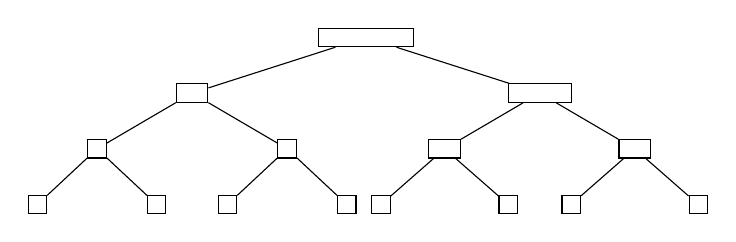
\begin{tikzpicture}[level distance=3cm,
  level 1/.style={sibling distance=12cm},
  level 2/.style={sibling distance=6cm}]
 \node [rectangle, minimum width=1.2cm, minimum height=0.2cm, draw] (root) {};
 \node [rectangle, minimum width=0.4cm, minimum height=0.2cm, below left   of=root,   xshift=-1.5cm,  draw] (left1)  {};
 \node [rectangle, minimum width=0.8cm, minimum height=0.2cm, below right  of=root,   xshift=1.5cm,   draw] (right1) {};
 \node [rectangle, minimum width=0.2cm, minimum height=0.2cm, below left   of=left1,  xshift=-0.5cm,  draw] (left2)  {};
 \node [rectangle, minimum width=0.2cm, minimum height=0.2cm, below right  of=left1,  xshift=0.5cm,   draw] (right2) {};
 \node [rectangle, minimum width=0.4cm, minimum height=0.2cm, below left   of=right1, xshift=-0.5cm,  draw] (left3)  {};
 \node [rectangle, minimum width=0.4cm, minimum height=0.2cm, below right  of=right1, xshift=0.5cm,   draw] (right3) {};
 \node [rectangle, minimum width=0.1cm, minimum height=0.2cm, below left   of=left2,  xshift=-0.05cm, draw] (left4)  {};
 \node [rectangle, minimum width=0.1cm, minimum height=0.2cm, below right  of=left2,  xshift=0.05cm,  draw] (right4) {};
 \node [rectangle, minimum width=0.1cm, minimum height=0.2cm, below left   of=right2, xshift=-0.05cm, draw] (left5)  {};
 \node [rectangle, minimum width=0.1cm, minimum height=0.2cm, below right  of=right2, xshift=0.05cm,  draw] (right5) {};
 \node [rectangle, minimum width=0.2cm, minimum height=0.2cm, below left   of=left3,  xshift=-0.1cm,  draw] (left6)  {};
 \node [rectangle, minimum width=0.2cm, minimum height=0.2cm, below right  of=left3,  xshift=0.1cm,   draw] (right6) {};
 \node [rectangle, minimum width=0.2cm, minimum height=0.2cm, below left   of=right3, xshift=-0.1cm,  draw] (left7)  {};
 \node [rectangle, minimum width=0.2cm, minimum height=0.2cm, below right  of=right3, xshift=0.1cm,   draw] (right7) {}; 
  \draw (root) -- (left1);
  \draw (root) -- (right1);
  \draw (left1) -- (left2);
  \draw (left1) -- (right2);
  \draw (right1) -- (left3);
  \draw (right1) -- (right3);
  \draw (left2) -- (left4);
  \draw (left2) -- (right4);
  \draw (right2) -- (left5);
  \draw (right2) -- (right5);
  \draw (left3) -- (left6);
  \draw (left3) -- (right6);
  \draw (right3) -- (left7);
  \draw (right3) -- (right7);
\end{tikzpicture}
}
\caption{ 
The tree matches the recursive calls made by \Cref{alg:unmerge}. Each node presents a rectangle with a length equal to the array given as input to the recursive call. The length of all the elements in a single level is equal to the original array length, thus we have that the linear work in each level sums up to $\Theta(n)$.
}
\end{figure}
\ifdefined\BOOK


\section{Appendix. Recursive Functions In Computer Science. (Beyond the scope of the 2024 course.)}


%\ctt{The current section repeats over part of the content above as it was designed to be self-contained. Also, notice that this part is considered as optional material and you are not required to remember the following algorithms for the final exam. Its primary goal is to expose you to "strange" running times. }


\begin{example}[Leading Example. numbers multiplication.]
Let \(x,y\) be an \(n\)'th digits numbers over \( \mathbb{F}^{n}_{2} \). It's known that summing such a pair requires a linear number of operations. Write an algorithm that calculates the multiplication \(x\cdot y\). 
\end{example}
\begin{example}[Long multiplication.]
To understand the real power of the dividing and conquer method, let's first examine the known solution from elementary school.  In that technics, we calculate the power order and the value of the digit separately and sum up the results at the end. Formally: \(x \leftarrow \sum_{i=0}^{n}{x_{i}2^{i}}\) Thus, \[ x\cdot y =\left( \sum_{i=0}^{n}{x_{i}2^{i}} \right) \left( \sum_{i=0}^{n}{y_{i}2^{i}} \right) =  \sum_{i,j \in [n]\times[n] }{ x_{i}y_{j}2^{i+j} }\] the above is a sum up over \(n^2\) numbers, each at length \(n\) and therefore the total running time of the algorithm is bounded by \( \theta(n^3) \). \ctt{ notice that adding \(1\) to \(1111111111...1\) requires \(O(n)\) }.
\end{example}
\begin{example}[Recursive Approach.] We could split \(x\) into the pair \(x_{l}, x_{r}\) such that \(x = x_{l} + 2^{\frac{n}{2}}x_{r} \). Then the multiplication of two \(n\)-long numbers will be reduced to sum up over multiplication of a quartet. Each at length \(\frac{n}{2}\). Thus, the running time is given by \begin{equation*}
    \begin{split}
 x\cdot y & = \left(x_{l} + 2^{\frac{n}{2}}x_{r}\right)\left(y_{l} + 2^{\frac{n}{2}}y_{r}\right) = x_{l}y_{l} + 2^{\frac{n}{2}} \left( x_{l}y_{r} + x_{r}y_{l} \right) + 2^{n}x_{r}y_{r} \\ &  \Rightarrow T\left(n\right)  =4T\left(\frac{n}{2}\right)+c\cdot n=4\cdot4T\left(\frac{n}{4}\right)+4c\cdot\frac{n}{2}+c\cdot n = ... = \\ & c\cdot n\left(1+\frac{4}{2}+\left(\frac{4}{2}\right)^{2}...+\left(\frac{4}{2}\right)^{h-1}\right) + 4^{h}T(1) = n^{2} + c\cdot n\cdot\frac{2^{h}-1}{2-1}
    \end{split}
\end{equation*}
We will call the number of iteration till the stopping condition the recursion height, and we will denote it by \(h\) . What should be the recursion height? \( 2^{h} = n \Rightarrow h =\log\left(n\right) \). So in total we get that multiplication could be achieved by performs \( \Theta\left(n^2\right)\) operations. 
\end{example}
\paragraph{Karatsuba algorithm.}
%Many years it was believed that multiplication can't done by less then $\Omega\left(n^2\right)$ time; until Karatsuba found the following algorithm \cite{Karatsuba1963MultiplicationOM}. Let $z_{0},z_{1}z_{3}$ defined as follow: \begin{equation*}
It was once thought that multiplication could not be done in less than $\Omega\left(n^2\right)$ time; however, Karatsuba discovered an algorithm \cite{Karatsuba1963MultiplicationOM} that proved this wrong. Let $z_{0},z_{1}z_{3}$ be defined as follows:
\begin{equation*}
z_0, z_1, z_2 \leftarrow x_{l}y_{r}, x_{l}y_{r} + x_{r}y_{l}, x_{r}y_{r}
\end{equation*}Notice that \( z_1 = \left(x_{l}+x_{r}\right)\left(y_{l}+y_{r}\right) - z_{0} -z_{1} \). summarize the above yields the following pseudo code. 

%{Karatsuba alg.}
\begin{algorithm}
\SetAlgoLined
\KwResult{returns the multiplication \(x\cdot y\) where \(x,y \in \mathbb{F}^{n}_{2}\) }
 \ \\ 
 \If{ \(x,y \in \mathbb{F}_{2}\) }
    { return \(x \cdot y\) } 
 \ \\ 
 
 \Else {
 define \(x_{l} , x_{r} \leftarrow x \) and \(y_{l} , y_{r} \leftarrow x \) \ \ \ \ \ // \( O \left(n\right) \). \\ 
 \ \\ 
 calculate \(z_0 \leftarrow \text{Karatsuba}\left(x_{l},y_{l}\right)\) \\
 \ \ \ \ \ \ \ \ \ \ \ \ \(z_2 \leftarrow \text{Karatsuba}\left(x_{r},y_{r}\right)\) \\ 
 \ \ \ \ \ \ \ \ \ \ \ \ \(z_1 \leftarrow \text{Karatsuba}\left(x_{r} + x_{l} ,y_{l} + y_{r} \right) - z_0 - z_2 \) \\ 
 \ \\
 return \(z_0 + 2^{\frac{n}{2}}z_1 + 2^{n}z_2\) \ \ \ \ \  // \( O \left(n\right) \). 
 }
\end{algorithm}
%
Let's analyze the running time of the algorithm above, assume that \(n = 2^{m}\) and then the recursive relation is 
\begin{equation*}
    \begin{split}
        T\left(n\right) & = 3T\left(\frac{n}{2}\right) + c\cdot n = 3^2 T\left(\frac{n}{2^2}\right) + \frac{3}{2}cn + c\cdot n = cn\left(1 + \frac{3}{2} + \left(\frac{3}{2}\right)^2 + ...  + \left(\frac{3}{2}\right)^{h-1} \right) + ) + 3^{h}T(1) \\
        & h = \log_{2}\left(n\right) \Rightarrow T\left(n\right) = n^{\log_{2}{3}} +  c\cdot \textcolor{red}{n}\cdot \left(\left(\frac{3}{\textcolor{red}{2}}\right)^{\log_{2}{n}}\right) / \left(\frac{3}{2} - 1\right) = \theta \left( 3^{\log_{2}(n)} \right) =  \theta \left( n^{\log 3} \right)  
    \end{split}
\end{equation*}
where \(n^{\log 3}  \sim n^{1.58} < n^2 \).

\fi




\newpage\chapter{Heaps - Recitation 4} 
\author{Correctness, Loop Invariant And Heaps.}


%\begin{paragraph}
  Apart from quantifying the resource requirement of our algorithms, we are also interested in proving that they indeed work. In this Recitation, we will demonstrate how to prove correctness via the notation of loop invariant. In addition, we will present the first (non-trivial) data structure in the course and prove that it allows us to compute the maximum efficiently.

%\end{paragraph}


\subsection*{Correctness And Loop Invariant.}
In this course, any algorithm is defined relative to a task/problem/function, And it will be said correctly if, for any input, it computes desirable output. For example, suppose that our task is to extract the maximum element from a given array. 
So the input space is all the arrays of numbers, and proving that a given algorithm is correct requires proving that the algorithm's output is the maximal number for an arbitrary array. Formally:  
\begin{defbox}{Correctness.}
We will say that an algorithm \( \mathcal{A}\) (an ordered set of operations) computes \( f:D_1 \rightarrow D_2 \) if for every \(x \in D_1 \Rightarrow f(x) = \mathcal{A}(x)\). Sometimes when it's obvious what is the goal function \(f\), we will abbreviate and say that \( \mathcal{A}\) is correct.       
\end{defbox}
\paragraph{}
Other functions \(f\) might be including any computation task: file saving, summing numbers, posting a message in the forum, etc. Let's dive back into the maximum extraction problem and see how one should prove correctness in practice.     
\paragraph{Task: Maximum Finding.} \textit{Given $n\in \mathbb{N}$ numbers $a_1, a_2, \cdots a_n \in \mathbb{R}$ write an Algorithm that returns their maximum.} 

Consider the following suggestion. How would you prove it correct?  
{Maximum finding.}
\begin{algorithm*}[H]
% \SetAlgoLined
 \SetKwInOut{Input}{input}
 \Input{ Array  $ a_1, a_2, .. a_n $  }
 let \(b \leftarrow a_1 \) \\ 
 \For{\(i \in [2, n] \) } { 
        \(b \leftarrow \max \left(b, a_i \right) \)
    } 
 return \( b \) 
 %\caption{maximum alg.}
\end{algorithm*}

Usually, it will be convenient to divide the algorithms into subsections and then characterize and prove their correctness separately. One primary technique is using the notation of Loop Invariant. Loop Invariant is a property that is characteristic of a loop segment code  and satisfies the following conditions:
\begin{defbox}{Loop Invariant.} 
\begin{enumerate}
  \item Initialization. The property holds (even) before the first iteration of the loop.    
    \item Conservation. As long as one performs the loop iterations, the property still holds.
    \item Termination. Exiting from the loop carrying information.
\end{enumerate}
\end{defbox}

Let's denote by $b^{(i)}$ the value of $b$ at line number $2$ at the $i$th iteration for $i\ge2$ and define $b^{(1)}$ to be its value in its initialization. What is the Loop Invariant here? \textbf{Claim.} \textit{"at the \(i\)-th iteration, $b^{(i)} = \max{ \{ a_1 ... a_{i} \} } $"}. 
\paragraph{Proof.} Initialization, clearly, $ b^{(1)} = a_{1} = \max{ \{ a_1 \} } $. Conservation, by induction, we have the base case from the initialization part, assume the correctness of the claim for any $i^\prime < i$, and consider the $i$th iteration (of course, assume that $i<n$). Then:  
\begin{equation*}
  \begin{split}
b^{(i)} = \max{ \{ b^{(i-1)}, a_{i} \} } = \max{ \{ \max{ \{ a_1, .. a_{i-2}, a_{i-1} \} }, a_{i} \} } = \max{ \{  a_{1}, .. a_{i} \} }
  \end{split}
\end{equation*} 
And that completes the Conservation part. Termination, followed by the conservation, at the $n$ iteration, $b^{(i)}$ is seted to $\max{ \{ a_1 ,a_2 .. a_n  \}}$. 

\paragraph{Task: Element finding.}  \textit{Given $n\in \mathbb{N}$ numbers $a_1, a_2, \cdots a_n \in \mathbb{R}$ and additional number $x \in \mathbb{R}$ write an Algorithm that returns $i$ s.t $a_{i} = x$ if there exists such $i$ and} False \textit{otherwise.} 

{Element finding.}
\begin{algorithm}[H]
\SetKwInOut{Input}{input}
 \Input{ Array  $ a_1, a_2, .. a_n $  }
% \SetAlgoLined
 \For{ \(i \in [n] \) } { 
	\If { \(a_{i} = x\) }{
	  return \(i, a_{i}\)
        }
    } 
    return False 
\end{algorithm}

\paragraph{Correctness Proof.} First, let's prove the following loop invariant. 
\subparagraph{Claim} \textit{Suppose that the running of the algorithm reached the i-th iteration, then $x \notin \{ a_{1} .. a_{i-1} \}$.} 
\textbf{Proof.} Initialization, for $i=1$ the claim is trivial. Let's use that as the induction base case for proving Conservation. Assume the correctness of the claim for any $i^{\prime} < i$. And consider the $i$th iteration. By the induction assumption, we have that $x \notin \{a_1 .. a_{i-2} \} $, and by the fact that we reached the $i$th iteration, we have that in the $i-1$ iteration, at the line (2) the conditional weren't satisfied (otherwise, the function would return at line (3) namely $x \neq a_{i-1}$. Hence, it follows that $ x \notin \{ a_1, a_2 .. a_{i-2}, a_{i-1} \} $.     
  \subparagraph{} Separate to cases. First, consider the case that given the input $a_1 .. a_n$, the algorithm return False. In this case, we have by the termination property that $x \notin \{ a_1 .. a_n \} $. Now, Suppose that the algorithm returns the pair $\left( i, x \right)$, then it means that the conditional at the line (2) was satisfied at the $i$th iteration. So, indeed $a_{i} = x$, and the algorithm returns the expected output.        


  \newpage
\subsection*{Heaps.}
  \paragraph{Task: The Superpharm Problem. (Motivation for Heaps) }\textit{You are requested to maintain a pharmacy line. In each turn, you get one of the following queries, either a new customer enters the shop, or the pharmacist requests the next person to stand in front. In addition, different customers have different priorities, So you are asked to guarantee that in each turn, the person with the height priority will be at the front.}

Before we consider a sophisticated solution, What is the running time for the naive solution? (maintaining the line as a linear array) ($\sim O\left( n^2 \right)$).

Heaps are structures that enable computing the maximum efficiency in addition to supporting adding and removing elements.
We have seen in the Lecture that no Algorithm can compute the $\max$ function with less than $n-1$ comparisons. So our solution above is indeed the best we could expect for. The same is true for the element-finding problem. Yet, we saw that if we are interested in storing the numbers, then, by keeping them according to sorted order, we could compute each query in logarithmic time via binary search. That raises the question, is it possible to have a similar result regarding the max problem?

\begin{defbox}{Heap}
  Let $n \in \mathbb{N}$ and consider the sequence $H = H_{1}, H_{2} \cdots H_{n} \in \mathbb{R} \left( * \right)$. we will say that $H$ is a Heap if for every $i \in [n]$ we have that: $H_{i} \le H_{2i}, H_{2i + 1}$ when we think of the value at indices greater than $n$ as $H_{i>n} = -\infty$. 
  \begin{equation*}
    \begin{split}
      \Leftrightarrow
    \end{split}
  \end{equation*}
  That definition is equivalent to the following recursive definition: Consider a binary tree in that we associate a number for each node. Then, we will say that this binary tree is a heap if the root's value is lower than its sons' values, and each subtree defined by its children is also a heap. 
\end{defbox}


    % Drawing a graph using the PG 3.0 graphdrawing library
% Author: Mark Wibrow
%\documentclass[tikz,border=10pt]{article}
%\usepackage{tikz}
%\usetikzlibrary{positioning}
%\begin{document}

\tikzset{%
  every neuron/.style={
    circle,
    draw,
    %fill=black,
    radius=0.05mm
  },
  neuron missing/.style={
    draw=none,
    scale=2,
    text height=0.25cm,
    execute at begin node=\color{black}$\vdots$
  },
}

\begin{tikzpicture}
    \node [every  neuron ] (v-1) at ( 0.0 ,-0) { $1$  };\node [every  neuron ] (v-2) at ( 0.0 ,-1) { $2$  };\node [every  neuron ] (v-3) at ( 4.0 ,-1) { $3$  };\node [every  neuron ] (v-4) at ( 0.0 ,-2) { $4$  };\node [every  neuron ] (v-5) at ( 2.0 ,-2) { $5$  };\node [every  neuron ] (v-6) at ( 4.0 ,-2) { $6$  };\node [every  neuron ] (v-7) at ( 6.0 ,-2) { $7$  };\node [every  neuron ] (v-8) at ( 0.0 ,-3) { $8$  };\node [every  neuron ] (v-9) at ( 1.0 ,-3) { $9$  };\node [every  neuron ] (v-10) at ( 2.0 ,-3) { $10$  };\node [every  neuron ] (v-11) at ( 3.0 ,-3) { $11$  };\node [every  neuron ] (v-12) at ( 4.0 ,-3) { $12$  };\node [every  neuron ] (v-13) at ( 5.0 ,-3) { $13$  };\node [every  neuron ] (v-14) at ( 6.0 ,-3) { $14$  };\node [every  neuron ] (v-15) at ( 7.0 ,-3) { $15$  };\draw [->] (v-1) -- (v-2);\draw [->] (v-1) -- (v-3);\draw [->] (v-2) -- (v-4);\draw [->] (v-2) -- (v-5);\draw [->] (v-3) -- (v-6);\draw [->] (v-3) -- (v-7);\draw [->] (v-4) -- (v-8);\draw [->] (v-4) -- (v-9);\draw [->] (v-5) -- (v-10);\draw [->] (v-5) -- (v-11);\draw [->] (v-6) -- (v-12);\draw [->] (v-6) -- (v-13);\draw [->] (v-7) -- (v-14);\draw [->] (v-7) -- (v-15);\end{tikzpicture}
\paragraph{Checking vital signs.}Are the following sequences are heaps? 
\begin{enumerate}
  \item 1,2,3,4,5,6,7,8,9,10 (Y)
  \item 1,1,1,1,1,1,1,1,1,1  (Y)
  \item 1,4,3,2,7,8,9,10     (N)
  \item 1,4,2,5,6,3	     (Y)
\end{enumerate}
\begin{figure}[h]
  \centering
  \begin{subfigure}[b]{0.3\textwidth}
	
    % Drawing a graph using the PG 3.0 graphdrawing library
% Author: Mark Wibrow
%\documentclass[tikz,border=10pt]{article}
%\usepackage{tikz}
%\usetikzlibrary{positioning}
%\begin{document}

\tikzset{%
  every neuron/.style={
    circle,
    draw,
    %fill=black,
    radius=0.05mm
  },
  neuron missing/.style={
    draw=none,
    scale=2,
    text height=0.25cm,
    execute at begin node=\color{black}$\vdots$
  },
}

\begin{tikzpicture}
    \node [every  neuron ] (v-1) at ( 0.0 ,-0) { $1$  };\node [every  neuron ] (v-2) at ( 0.0 ,-1) { $1$  };\node [every  neuron ] (v-3) at ( 2.5 ,-1) { $1$  };\node [every  neuron ] (v-4) at ( 0.0 ,-2) { $1$  };\node [every  neuron ] (v-5) at ( 1.25 ,-2) { $1$  };\node [every  neuron ] (v-6) at ( 2.5 ,-2) { $1$  };\node [every  neuron ] (v-7) at ( 3.75 ,-2) { $1$  };\node [every  neuron ] (v-8) at ( 0.0 ,-3) { $1$  };\node [every  neuron ] (v-9) at ( 0.625 ,-3) { $1$  };\draw [->] (v-1) -- (v-2);\draw [->] (v-1) -- (v-3);\draw [->] (v-2) -- (v-4);\draw [->] (v-2) -- (v-5);\draw [->] (v-3) -- (v-6);\draw [->] (v-3) -- (v-7);\draw [->] (v-4) -- (v-8);\draw [->] (v-4) -- (v-9);\end{tikzpicture}
  \end{subfigure}
\begin{subfigure}[b]{0.3\textwidth}
	
    % Drawing a graph using the PG 3.0 graphdrawing library
% Author: Mark Wibrow
%\documentclass[tikz,border=10pt]{article}
%\usepackage{tikz}
%\usetikzlibrary{positioning}
%\begin{document}

\tikzset{%
  every neuron/.style={
    circle,
    draw,
    %fill=black,
    radius=0.05mm
  },
  neuron missing/.style={
    draw=none,
    scale=2,
    text height=0.25cm,
    execute at begin node=\color{black}$\vdots$
  },
}

\begin{tikzpicture}
    \node [every  neuron ] (v-1) at ( 0.0 ,-0) { $1$  };\node [every  neuron, fill=black,  text=white, draw=black ] (v-2) at ( 0.0 ,-1) { $4$  };\node [every  neuron ] (v-3) at ( 2.0 ,-1) { $3$  };\node [every  neuron ] (v-4) at ( 0.0 ,-2) { $2$  };\node [every  neuron ] (v-5) at ( 1.0 ,-2) { $7$  };\node [every  neuron ] (v-6) at ( 2.0 ,-2) { $8$  };\node [every  neuron ] (v-7) at ( 3.0 ,-2) { $9$  };\draw [->] (v-1) -- (v-2);\draw [->] (v-1) -- (v-3);\draw [->] (v-2) -- (v-4);\draw [->] (v-2) -- (v-5);\draw [->] (v-3) -- (v-6);\draw [->] (v-3) -- (v-7);\end{tikzpicture}

  \end{subfigure}
\begin{subfigure}[b]{0.3\textwidth}
	
    % Drawing a graph using the PG 3.0 graphdrawing library
% Author: Mark Wibrow
%\documentclass[tikz,border=10pt]{article}
%\usepackage{tikz}
%\usetikzlibrary{positioning}
%\begin{document}

\tikzset{%
  every neuron/.style={
    circle,
    draw,
    %fill=black,
    radius=0.05mm
  },
  neuron missing/.style={
    draw=none,
    scale=2,
    text height=0.25cm,
    execute at begin node=\color{black}$\vdots$
  },
}

\begin{tikzpicture}
    \node [every  neuron ] (v-1) at ( 0.0 ,-0) { $1$  };\node [every  neuron ] (v-2) at ( 0.0 ,-1) { $4$  };\node [every  neuron ] (v-3) at ( 1.5 ,-1) { $2$  };\node [every  neuron ] (v-4) at ( 0.0 ,-2) { $5$  };\node [every  neuron ] (v-5) at ( 0.75 ,-2) { $6$  };\draw [->] (v-1) -- (v-2);\draw [->] (v-1) -- (v-3);\draw [->] (v-2) -- (v-4);\draw [->] (v-2) -- (v-5);\end{tikzpicture}
  \end{subfigure}
  \caption{The trees representations of the heaps above. The node which fails to satisfy the Heap inequality is colorized.}
\end{figure}
How much is the cost (running time) to compute the min of $H$? (without changing the heap). ($O\left( 1 \right)$). Assume that option 4 is our Superpharm Line. Let's try to imagine how we should maintain the line. After serving the customer at the top, what can be said on $ \{ H_{2}, H_{3}\}$? or $\{H_{i>3}\}?$ (the second highest value is in $\{H_{2}, H_{3} \}$.)   
\paragraph{Subtask: Extracting Heap's Minimum.} \textit{Let $H$ be an Heap at size $n$, Write algorithm which return $H_1$, erase it and returns $H^\prime$, an Heap which contain all the remain elements.} 
\textbf{Solution:} 

{Extract-min.}
\begin{algorithm}[H]
\SetKwInOut{Input}{input}
 \Input{ Heap  $ H_1, H_2, .. H_n $  }
% \SetAlgoLined
ret $\leftarrow H_{1} $ \\
$ H_{1} \leftarrow H_{n} $  \\
$ n \leftarrow n -1 $ \\
Heapify-down$\left( 1 \right)$ \\
return ret  
\end{algorithm}




{Heapify-down.}
\begin{algorithm}[H]
\SetKwInOut{Input}{input}
 \Input{ Array  $ a_1, a_2, .. a_n $  }
% \SetAlgoLined
next  $\leftarrow i  $ \\
left  $\leftarrow 2i $ \\
right $\rightarrow 2i +1 $ \\ 
\If{ left $ < n \text{ and }  H_{\text{left}} < H_{\text{next}}$ } {
  next $\leftarrow$ left 
}
\If{ right $ < n \text{ and }  H_{\text{right}} < H_{\text{next}}$ } {
  next $\leftarrow$  right
}
\If{ $ i \neq $ next } {
  $ H_{i} \leftrightarrow H_{\text{next}} $ \\ 
  Heapify-down$\left( \text{next}  \right)$
}
\end{algorithm}


 

\begin{figure}[h]
  \centering
  \begin{subfigure}[b]{0.23\textwidth}
	
    % Drawing a graph using the PG 3.0 graphdrawing library
% Author: Mark Wibrow
%\documentclass[tikz,border=10pt]{article}
%\usepackage{tikz}
%\usetikzlibrary{positioning}
%\begin{document}

\tikzset{%
  every neuron/.style={
    circle,
    draw,
    %fill=black,
    radius=0.1mm
  },
  neuron missing/.style={
    draw=none,
    scale=2,
    text height=0.25cm,
    execute at begin node=\color{black}$\vdots$
  },
}

\begin{tikzpicture}
    \node [every  neuron ] (v-1) at ( 0.0 ,-0) { $1$  };
  \node [every  neuron ] (v-2) at ( 0.0 ,-1) { $4$  };
\node [every  neuron ] (v-3) at ( 1.5 ,-1) { $2$  };
\node [every  neuron ] (v-4) at ( 0.0 ,-2) { $5$  };
\node [every  neuron ] (v-5) at ( 0.75 ,-2) { $6$  };
\node [every  neuron ] (v-6) at ( 1.5 ,-2) { $2$  };
\node [every  neuron ] (v-7) at ( 2.25 ,-2) { $3$  };
\draw [->] (v-1) -- (v-2);
\draw [->] (v-1) -- (v-3);
\draw [->] (v-2) -- (v-4);
\draw [->] (v-2) -- (v-5);
\draw [->] (v-3) -- (v-6);
\draw [->] (v-3) -- (v-7);
\end{tikzpicture} 

  \end{subfigure}
\begin{subfigure}[b]{0.23\textwidth}
	
    % Drawing a graph using the PG 3.0 graphdrawing library
% Author: Mark Wibrow
%\documentclass[tikz,border=10pt]{article}
%\usepackage{tikz}
%\usetikzlibrary{positioning}
%\begin{document}

\tikzset{%
  every neuron/.style={
    circle,
    draw,
    %fill=black,
    radius=0.1mm
  },
  neuron missing/.style={
    draw=none,
    scale=2,
    text height=0.25cm,
    execute at begin node=\color{black}$\vdots$
  },
}

\begin{tikzpicture}
    \node [every  neuron ] (v-1) at ( 0.0 ,-0) { $3$  };
  \node [every  neuron ] (v-2) at ( 0.0 ,-1) { $4$  };
\node [every  neuron ] (v-3) at ( 1.5 ,-1) { $2$  };
\node [every  neuron ] (v-4) at ( 0.0 ,-2) { $5$  };
\node [every  neuron ] (v-5) at ( 0.75 ,-2) { $6$  };
\node [every  neuron ] (v-6) at ( 1.5 ,-2) { $2$  };
\draw [->] (v-1) -- (v-2);
\draw [->] (v-1) -- (v-3);
\draw [->] (v-2) -- (v-4);
\draw [->] (v-2) -- (v-5);
\draw [->] (v-3) -- (v-6);
\end{tikzpicture} 

  \end{subfigure}
\begin{subfigure}[b]{0.23\textwidth}
	
    % Drawing a graph using the PG 3.0 graphdrawing library
% Author: Mark Wibrow
%\documentclass[tikz,border=10pt]{article}
%\usepackage{tikz}
%\usetikzlibrary{positioning}
%\begin{document}

\tikzset{%
  every neuron/.style={
    circle,
    draw,
    %fill=black,
    radius=0.1mm
  },
  neuron missing/.style={
    draw=none,
    scale=2,
    text height=0.25cm,
    execute at begin node=\color{black}$\vdots$
  },
}

\begin{tikzpicture}
    \node [every  neuron ] (v-1) at ( 0.0 ,-0) { $2$  };
  \node [every  neuron ] (v-2) at ( 0.0 ,-1) { $4$  };
\node [every  neuron ] (v-3) at ( 1.5 ,-1) { $3$  };
\node [every  neuron ] (v-4) at ( 0.0 ,-2) { $5$  };
\node [every  neuron ] (v-5) at ( 0.75 ,-2) { $6$  };
\node [every  neuron ] (v-6) at ( 1.5 ,-2) { $2$  };
\draw [->] (v-1) -- (v-2);
\draw [->] (v-1) -- (v-3);
\draw [->] (v-2) -- (v-4);
\draw [->] (v-2) -- (v-5);
\draw [->] (v-3) -- (v-6);
\end{tikzpicture}

  \end{subfigure}
\begin{subfigure}[b]{0.23\textwidth}
	
    % Drawing a graph using the PG 3.0 graphdrawing library
% Author: Mark Wibrow
%\documentclass[tikz,border=10pt]{article}
%\usepackage{tikz}
%\usetikzlibrary{positioning}
%\begin{document}

\tikzset{%
  every neuron/.style={
    circle,
    draw,
    %fill=black,
    radius=0.1mm
  },
  neuron missing/.style={
    draw=none,
    scale=2,
    text height=0.25cm,
    execute at begin node=\color{black}$\vdots$
  },
}

\begin{tikzpicture}
    \node [every  neuron ] (v-1) at ( 0.0 ,-0) { $2$  };\node [every  neuron ] (v-2) at ( 0.0 ,-1) { $4$  };\node [every  neuron ] (v-3) at ( 1.5 ,-1) { $2$  };\node [every  neuron ] (v-4) at ( 0.0 ,-2) { $5$  };\node [every  neuron ] (v-5) at ( 0.75 ,-2) { $6$  };\node [every  neuron ] (v-6) at ( 1.5 ,-2) { $3$  };\draw [->] (v-1) -- (v-2);\draw [->] (v-1) -- (v-3);\draw [->] (v-2) -- (v-4);\draw [->] (v-2) -- (v-5);\draw [->] (v-3) -- (v-6);\end{tikzpicture}
  \end{subfigure}
  \caption{Running Example, Extract.} 
\end{figure}


\paragraph{Claim.} Assume that $H$ satisfies the Heap inequality for all the elements except the root. Namely for any $i \neq 1$ we have that $H_{i} \le H_{2i}, H_{2i+1}$. Then applying Heapify-down on $H$ at index $1$ returns a heap.  
\paragraph{Proof.} By induction on the heap size.  
 
\begin{itemize} 
  \item Base, Consider a heap at the size at most three and prove for each by considering each case separately. (lefts as exercise).  
  \item Assumption, assume the correctness of the Claim for any tree that satisfies the heap inequality except the root, at size $n^{\prime} < n$. 
  \item Induction step. Consider a tree at size $n$ which and assume w.l.g (why could we?) that the right child of the root is the minimum between the triple. Then, by the definition of the algorithm, at line 9, the root exchanges its value with its right child. Given that before the swapping, all the elements of the heap, except the root, had satisfied the heap inequality, we have that after the exchange, all the right subtree's elements, except the root of that subtree (the original root's right child) still satisfy the inequality. As the size of the right subtree is at most $n-1$, we could use the assumption and have that after line (10), the right subtree is a heap.  
 
    Now, as the left subtree remains the same (the values of the nodes of the left side didn't change), we have that this subtree is also a heap. So it's left to show that the new tree's root is smaller than its children's. Suppose that is not the case, then it's clear that the root of the right subtree (heap) is smaller than the new root. Combining the fact that its origin must be the right subtree, we have a contradiction to the fact that the original right subtree was a heap (as its root wasn't the minimum element in that subtle).  
 
\end{itemize} 
\paragraph{Question.} How to construct a heap? And how much time will it take?   
{Build.}
\begin{algorithm}[H]
  \SetKwInOut{Input}{input}
% \SetAlgoLined
  \Input{ Array $ H = H_{1} .. H_{n} $ }
  $ i \leftarrow \lfloor \frac{1}{2}n  \rfloor $ \\
  \While { $ i > 1 $ }
  { 
    Heapify-down $\left( H, i \right)$ \\ 
    $ i \leftarrow i - 1 $  
  }
return $H_{1} .. H_{n}$
\end{algorithm}

We can compute a simple upper bound on the running time of Build as follows. Each call to Heapify costs $O(\log n)$ time, and Build makes $O(n)$ such calls. Thus, the running time is $O(n \log n)$. This upper bound, though correct, is not as tight as it can be.

Let's compute the tight bound. Denote by $U_h$ the subset of vertices in a heap at height $h_{i}$. Also, let $c > 0 $ be the constant quantify the work that is done in each recursive step, then we can express the total cost as being bonded from above by: 

\begin{equation*}
  \begin{split}
    T\left( n \right) & \le \sum_{ h_{i} =1}^{ \log n }{c \cdot \left( \log n -  h_{i} \right)  |U_{h_{i}}|   } 
  \end{split}
\end{equation*}

By counting arguments, we have the inequality $ 2^{\log n - h_{i}}|U_{i}| \le n $ (Proving this argument is left as an exercise). We thus obtain:  

\begin{equation*}
  \begin{split}
    T\left( n \right)  & \le  \sum_{ h_{i} =1}^{ \log n }{c \cdot \left( \log n -  h_{i} \right) \frac{n}{2^{log n - h_{i}} }} = c n \sum_{ j = 1}^{ \log n }{ 2^{-j} \cdot j  }  \\ 
      \le &  c n \sum_{ j = 1}^{ \infty }{ 2^{-j} \cdot j  } 
  \end{split}
\end{equation*}
And by the Ratio test for inifinte serires $ \lim_{j\rightarrow \infty} \frac{(j+1)2^{-j-1}}{j2^{-j}} \rightarrow \frac{1}{2}$ we have that the serire covergence to constant. Hence: $ T\left( n \right) = \Theta\left( n \right) $. 


\paragraph{Heap Sort.}   
Combining the above, we obtain a new sorting algorithm. Given an array, we could first Heapify it (build a heap from it) and then extract the elements by their order. As we saw, the construction requires linear time, and then each extraction costs $\log n$ time. So, the overall cost is $O\left( n\log n  \right)$. Correction follows immediately from Build and Extract correction.  
{Heap-Sort.}
\begin{algorithm}[H]
\SetKwInOut{Input}{input}
 \Input{ Array  $ H_1, H_2, .. H_n $  }
% \SetAlgoLined
  $H \leftarrow $ build $ \left( x_1, x_2 .. x_{n}  \right) $ \\ 
  ret $ \leftarrow $ Array $ \{ \} $ \\
  \For {  $ i \in [n] $ } {
  ret$_{i}$ $\leftarrow$ extract $H$
  }
  return ret. 
\end{algorithm}


\paragraph{Adding Elements Into The Heap.} (Skip if there is no time).

{Heapify-up.}
\begin{algorithm}[H]
  \SetKwInOut{Input}{input}
 \Input{ Heap  $ H_1, H_2, .. H_n $  }
% \SetAlgoLined
parent $\leftarrow \lfloor i/2 \rfloor $ \\
\If{ \text{parent} $  > 0 \text{ and }  H_{\text{parent}} \le H_{i}$ } { 
  $ H_{i} \leftrightarrow H_{\text{parent}} $ \\ 
  Heapify-up$\left( \text{parent}  \right)$
}
\end{algorithm}




{Insert-key.}
\begin{algorithm}[H]
\SetKwInOut{Input}{input}
 \Input{ Heap  $ H_1, H_2, .. H_n $  }
% \SetAlgoLined
$ H_{n} \leftarrow v $ \\ 
Heapify-up$\left( n \right)$\\
$ n \leftarrow n + 1 $ 
\end{algorithm}




\newpage 
\subsection*{Example, Median Heap}

\paragraph{Task:}Write a datastructure that support insertion and deltion at $O\left( \log n \right) $ time and in addition enable to extract the median in $O\left( \log n  \right)$ time. 

\paragraph{Soultlion.} We will define two separate Heaps, the first will be a maximum heap and store the first $ \lfloor n/2 \rfloor $ smallest elements, and the second will be a minimum heap and contain the $ \lceil n/2 \rceil$ greatest elements. So, it's clear that the root of the maximum heap is the median of the elements. Therefore to guarantee correctness, we should maintain the balance between the heap's size. Namely, promising that after each insertion or extraction, the difference between the heap's size is either $0$ or $1$.

{Median-Insert-key.}
\begin{algorithm}[H]  
\SetKwInOut{Input}{input} 
\Input{ Array  $ H_1, H_2, .. H_n , v $  } 
\If {$ H_{\max, 1} \le v \le  H_{\min, 1}$ } {
	\If{ size $(H_{\max}) - $ size$(H_{\min}) = 1$} {
       Insert-key ( $H_{min}$, $v$ )
    }
    \Else{
	    Insert-key ( $H_{max}$, $v$ )
    }
}
\Else{
median $\leftarrow$ Median-Extract $H$ \\
\If{ $v < $ median  }{
   Insert-key ( $H_{max}$, $v$ ) \\
   Insert-key ( $H_{min}$, $median$ ) \\
}
\Else{
   Insert-key ( $H_{min}$, $v$ ) \\
   Insert-key ( $H_{max}$, $median$ ) \\
}
}
\end{algorithm}


{Median-Extract.}
\begin{algorithm}[H]
\SetKwInOut{Input}{input}
 \Input{ Array  $ H_1, H_2, .. H_n $  }
% \SetAlgoLined
median $\leftarrow$ extract $H_{max}$ \\   
\If{ size($H_{min}$) - size($H_{max}$) $> 0$ }{
  temp $ \leftarrow $ extract $H_{\min}$ \\
  Insert-key ( $H_{max}$, temp )    \\
}
return median 
\end{algorithm}


\begin{figure}[h]
  \centering
  \begin{subfigure}[b]{0.49\textwidth}
	
    % Drawing a graph using the PG 3.0 graphdrawing library
% Author: Mark Wibrow
%\documentclass[tikz,border=10pt]{article}
%\usepackage{tikz}
%\usetikzlibrary{positioning}
%\begin{document}

\tikzset{%
  every neuron/.style={
    circle,
    draw,
    %fill=black,
    radius=0.1mm
  },
  neuron missing/.style={
    draw=none,
    scale=2,
    text height=0.25cm,
    execute at begin node=\color{black}$\vdots$
  },
}

\begin{tikzpicture}
    \node [every  neuron ] (v-1) at ( 0.0 ,-0) { $143$  };\node [every  neuron ] (v-2) at ( 0.0 ,-1) { $140$  };\node [every  neuron ] (v-3) at ( 4.0 ,-1) { $142$  };\node [every  neuron ] (v-4) at ( 0.0 ,-2) { $124$  };\node [every  neuron ] (v-5) at ( 2.0 ,-2) { $129$  };\node [every  neuron ] (v-6) at ( 4.0 ,-2) { $134$  };\node [every  neuron ] (v-7) at ( 6.0 ,-2) { $131$  };\node [every  neuron ] (v-8) at ( 0.0 ,-3) { $113$  };\node [every  neuron ] (v-9) at ( 1.0 ,-3) { $29$  };\node [every  neuron ] (v-10) at ( 2.0 ,-3) { $16$  };\node [every  neuron ] (v-11) at ( 3.0 ,-3) { $87$  };\node [every  neuron ] (v-12) at ( 4.0 ,-3) { $113$  };\node [every  neuron ] (v-13) at ( 5.0 ,-3) { $24$  };\node [every  neuron ] (v-14) at ( 6.0 ,-3) { $44$  };\node [every  neuron ] (v-15) at ( 7.0 ,-3) { $130$  };\node [every  neuron ] (v-16) at ( 0.0 ,-4) { $77$  };\node [every  neuron ] (v-17) at ( 1.0 ,-4) { $78$  };\draw [->] (v-1) -- (v-2);\draw [->] (v-1) -- (v-3);\draw [->] (v-2) -- (v-4);\draw [->] (v-2) -- (v-5);\draw [->] (v-3) -- (v-6);\draw [->] (v-3) -- (v-7);\draw [->] (v-4) -- (v-8);\draw [->] (v-4) -- (v-9);\draw [->] (v-5) -- (v-10);\draw [->] (v-5) -- (v-11);\draw [->] (v-6) -- (v-12);\draw [->] (v-6) -- (v-13);\draw [->] (v-7) -- (v-14);\draw [->] (v-7) -- (v-15);\draw [->] (v-8) -- (v-16);\draw [->] (v-8) -- (v-17);\end{tikzpicture}
  \end{subfigure}
\begin{subfigure}[b]{0.49\textwidth}
	
    % Drawing a graph using the PG 3.0 graphdrawing library
% Author: Mark Wibrow
%\documentclass[tikz,border=10pt]{article}
%\usepackage{tikz}
%\usetikzlibrary{positioning}
%\begin{document}

\tikzset{%
  every neuron/.style={
    circle,
    draw,
    %fill=black,
    radius=0.1mm
  },
  neuron missing/.style={
    draw=none,
    scale=2,
    text height=0.25cm,
    execute at begin node=\color{black}$\vdots$
  },
}

\begin{tikzpicture}
    \node [every  neuron ] (v-1) at ( 0.0 ,-0) { $185$  };\node [every  neuron ] (v-2) at ( 0.0 ,-1) { $209$  };\node [every  neuron ] (v-3) at ( 4.0 ,-1) { $223$  };\node [every  neuron ] (v-4) at ( 0.0 ,-2) { $229$  };\node [every  neuron ] (v-5) at ( 2.0 ,-2) { $217$  };\node [every  neuron ] (v-6) at ( 4.0 ,-2) { $242$  };\node [every  neuron ] (v-7) at ( 6.0 ,-2) { $280$  };\node [every  neuron ] (v-8) at ( 0.0 ,-3) { $254$  };\node [every  neuron ] (v-9) at ( 1.0 ,-3) { $315$  };\node [every  neuron ] (v-10) at ( 2.0 ,-3) { $218$  };\node [every  neuron ] (v-11) at ( 3.0 ,-3) { $291$  };\node [every  neuron ] (v-12) at ( 4.0 ,-3) { $281$  };\node [every  neuron ] (v-13) at ( 5.0 ,-3) { $296$  };\node [every  neuron ] (v-14) at ( 6.0 ,-3) { $282$  };\node [every  neuron ] (v-15) at ( 7.0 ,-3) { $291$  };\node [every  neuron ] (v-16) at ( 0.0 ,-4) { $330$  };\node [every  neuron ] (v-17) at ( 1.0 ,-4) { $307$  };\draw [->] (v-1) -- (v-2);\draw [->] (v-1) -- (v-3);\draw [->] (v-2) -- (v-4);\draw [->] (v-2) -- (v-5);\draw [->] (v-3) -- (v-6);\draw [->] (v-3) -- (v-7);\draw [->] (v-4) -- (v-8);\draw [->] (v-4) -- (v-9);\draw [->] (v-5) -- (v-10);\draw [->] (v-5) -- (v-11);\draw [->] (v-6) -- (v-12);\draw [->] (v-6) -- (v-13);\draw [->] (v-7) -- (v-14);\draw [->] (v-7) -- (v-15);\draw [->] (v-8) -- (v-16);\draw [->] (v-8) -- (v-17);\end{tikzpicture}
  \end{subfigure}
  \caption{ Example for Median-Heap, the left and right trees are maximum and minimum heaps.  }
\end{figure}

\iffalse 
  \newpage

\section{ Appendix. Exercise from last year }

\paragraph{Question.} Consider the sets $X = \{x_1,x_2 .. x_n\}$, $Y = \{y_1, y_2 .. y_n\}$. Assume that each of the values $x_i,y_i$ is unique. Write an Algorithm which compute the $k$ most small items in $X \oplus Y = \{ x_{i} + y_{j} : x_{i} \in X , y_{j} \in Y  \} $ at $ O \left( n + k\log k  \right) $ time. 

\textbf{Solution.} Notice that If $a \in X$ is greater than $i$ elements of $X$ and $b \in Y$ greater than $j$ elements of $Y$. Then, $a + b$  greater than $i\cdot j$ elements of $X \oplus Y$. Denote by $X^\prime = \{ x^{\prime}_{1} .. x^{\prime}_{n}$ ( $Y^{\prime}$ ) The elements of $X$ in sorted order. So it's clear that if $x_{i}+y_{j} = x^{\prime}_{i^{\prime}} + y^{\prime}_{j^{\prime}}$ is one of the $k$ smallest elements of $X\oplus Y$ then $i^{\prime}j^{\prime} \ge k$. So we will create a heap of elements that respect that inequality and then query that heap.

{Heappush.}
\begin{algorithm}[H]
% \SetAlgoLined
$ H_{X} \leftarrow $ build $\left( X \right)$  \\ 
$ H_{Y} \leftarrow $ build $\left( Y \right)$  \\
$ S_{X} \leftarrow $ extract-$k$ $\left( H_{X} \right)$  \\ 
$ S_{Y} \leftarrow $ extract-$k$ $\left( H_{Y} \right)$  \\
$ H_{XY} \leftarrow $ Heap $(\{ \} )$ \\
\For{ $i \in [k]$ } {
  \For { $j \in [k/i]$ } {
  	Heappush( $H_{XY}$, $S_{X,i} + S_{Y, j}$ )    
  }
}
return extract-$k$ ( $H_{XY}$ ) 
\end{algorithm}

\fi



\newpage\chapter{Quicksort And Liner Time Sorts  - Recitation 6} 
\author{Quicksort, Countingsort, Radixsort, And Bucketsort.}


%\begin{paragraph}
Till now, we have quantified the algorithm performance against the worst-case scenario. And we saw that according to that measure, In the comparisons model, one can not sort in less than $\Theta\left( n\log n \right) $ time. In this recitation, we present two new main concepts that, in some instances, achieve better analyses. The first one is the Exception Complexity; By Letting the algorithm behave non-determinately, we might obtain an algorithm that most of the time runs to compute the task fast. Yet we will not success get down beneath the $\Theta\left(n\log n\right)$ lower bound, but we will go back to use that concept in the pending of the course. The second concept is to restrict ourselves to dealing only with particular inputs. For example, We will see that if we suppose that the given array contains only integers in a bounded domain, then we can sort it in linear time.  

%\end{paragraph}

\subsection*{Quicksort.}
The quicksort algorithm is a good example of a \textbf{non-determistic} algorithm that has a worst-case running time of $\Theta\left(n^{2}\right)$. Yet its expected running time is $\Theta\left(n\log n\right)$. Namely, fix an array of $n$ numbers. The running of Quicksort over that array might be different. Each of them is a different event in probability space, and the algorithm's running time is a random variable defined over that space. Saying that the algorithm has the worst space complexity of $\Theta(n^{2})$ means that there exists an event in which it runs $\Theta\left(n^{2}\right)$ time with non-zero probability. But practically, the interesting question is not the existence of such an event but how likely it would happen. It turns out that the expectation of the running time is $\Theta\left(n\log n\right)$.  

What is the exact reason that happens? By giving up on the algorithm behavior century, we will turn the task of engineering a bad input impossible.    
 
{randomized-partition$(A, p, r)$}
  \begin{algorithm}[H]
      $i \leftarrow $ random $(p, r)$ \\
      $A_{r} \leftrightarrow A_{i} $ \\
      return Partition $(A, p, r)$
    \end{algorithm}

 {randomized-quicksort $(A, p, r)$}
      \begin{algorithm}[H]
	\If{ $p < r$ }{
	  $q \leftarrow $ randomized-partition $(A, p, r)$ \\
	  randomized-quicksort $(A, p, q-1)$\\
	  randomized-quicksort $(A, q+1, r)$
	}
      \end{algorithm}



\paragraph{Partitioning.}
To complete the correctness proof of the algorithm (most of it passed in the Lecture), we have to prove that the partition method is indeed rearranging the array such that all the elements contained in the right subarray are greater than all the elements on the left subarray.  

%which rearranges the subarray $ A_{p : r}$ in place, returning the index of the dividing point between the two sides of the partition.

{Partition$(A, p, r)$}
  \begin{algorithm}[H]
    $ x \leftarrow A_{r} $ \\
    $ i \leftarrow p - 1 $ \\
    \For{ $j \in [p, r-1]$ }{
      \If{ $ A_{j} \le x  $}{
	$ i \leftarrow i + 1 $ \\
	$ A_{i} \leftrightarrow A_{j} $\\
      }
    }
   $ A_{i+1} \leftrightarrow A_{r} $\\
   return $ i+1$
  \end{algorithm}


\paragraph{claim.} At the beginning of each iteration of the loop of lines 3–6, for any array index $k$, the following conditions hold:
\begin{itemize}
  \item  if $p \le k \le i$, then $A_{k} \le x$.
  \item  if $i + 1 \le k \le j – 1$, then $A_{k} > x$.
  \item  if $k = r$, then $A_{k} = x$.
\end{itemize}
\paragraph{Proof.}
\begin{enumerate}
  \item Initialization: Prior to the first iteration of the loop, we have $i = p – 1$ and $ j= p$. Because no values lie between $p$ and $i$ and no values lie between $i + 1$ and $j – 1$, the first two conditions of the loop invariant are trivially satisfied. The assignment in line 1 satisfies the third condition.
  \item Maintenance: we consider two cases, depending on the outcome of the test in line 4, when $A_{j} > x$: the only action in the loop is to increment $j$. After $j$  has been incremented, the second condition holds for $A_{j – 1}$, and all other entries remain unchanged. When $A_{j} \le x$: the loop increments $i$, swaps $A_{i}$ and $A_{j}$, and then increments $j$. Because of the swap, we now have that $A_{i} \le x$, and condition 1 is satisfied. Similarly, we also have that $A_{j – 1} > x$, since the item that was swapped into $A_{j – 1}$ is, by the loop invariant, greater than $x$.
  \item Termination: Since the loop makes exactly $r – p$ iterations, it terminates, whereupon$ j= r$. At that point, the unexamined subarray $A_{j}, A_{j+1}..  A_{r – 1}$ is empty, and every entry in the array belongs to one of the other three sets described by the invariant. Thus, the values in the array have been partitioned into three sets: those less than or equal to $x$ (the low side), those greater than $x$ (the high side), and a singleton set containing $x$ (the pivot).


\end{enumerate}


    % Drawing a graph using the PG 3.0 graphdrawing library
% Author: Mark Wibrow
%\documentclass[tikz,border=10pt]{article}
%\usepackage{tikz}
%\usetikzlibrary{positioning}
%\begin{document}

\newcommand{\vet}[1]{\foreach \num in {#1}{\el{\num}}}
\newcommand{\el}[1]{\tikz{\node[font=\footnotesize, minimum size=16pt, draw]{#1}}}
\newcommand{\bl}{\color{blue}}
\newcommand{\gr}{\color{gray}}
\newcommand{\re}{\color{red}}
\begin{tabular}{cccc}
    \vet{1, 5, 8, 5, 3, 2, 1} & &\vet{1, 1, 2, \re3, 5, 8, \re5} & \\ \vet{\bl1, 5, 8, 5, 3, 2, \bl1} & quicksort$(A,0,6)$&\vet{1, 1, 2, 3, \bl5, 8, \bl5} & quicksort$(A,4,6)$\\ \vet{\re1, 5, 8, 5, 3, 2, \re1} & &\vet{1, 1, 2, 3, 5, \re5, \re8} & \\ \vet{\re1, 5, 8, 5, 3, 2, 1} & &\vet{1, 1, 2, 3, \re5, 5, 8} & \\ \vet{1, \re1, 8, 5, 3, 2, \re5} & &\vet{1, 1, 2, 3, 5, \re5, 8} & \\ \vet{1, 1, \bl8, 5, 3, 2, \bl5} & quicksort$(A,2,6)$&\vet{1, 1, 2, 3, \bl5, \bl5, 8} & quicksort$(A,4,5)$\\ \vet{1, 1, 8, 5, \re5, 2, \re3} & &\vet{1, 1, 2, 3, \re5, \re5, 8} & \\ \vet{1, 1, \re2, 5, 5, \re8, 3} & &\vet{1, 1, 2, 3, \re5, 5, 8} & \\ \end{tabular}

\subsection*{Linear Time Sorts}
\paragraph{ Counting sort.} Counting sort assumes that each of the n input elements is an integer at the size at most $k$. It runs in $\Theta \left(n + k\right)$ time, so that when $k = O(n)$, counting sort runs in $\Theta\left(n\right)$ time.
Counting sort first determines, for each input element $x$, the number of elements less than or equal to $x$. It then uses this information to place element $x$ directly into its position in the output array. For example, if 17 elements are less than or equal to $x$, then $x$ belongs in output position 17. We must modify this scheme slightly to handle the situation in which several elements have the \textbf{same value}, since we do not want them all to end up in the same position.

{Counting-sort$(A, n, k)$}
  \begin{algorithm}[H]
  	let B and C be new arrays at size $n$ and $k$ \\ 
  	\For{ $i \in  [0, k]$}{
		$C_{i} \leftarrow 0 $
  	}
	\For{ $j \leftarrow [1, n]$}{
	  $C_{A{j}} \leftarrow C_{A_{j}} + 1 $
 	}
	\For{ $i \in  [1, k]$}{
	  $C_{i} \leftarrow C_{i} + C_{i – 1} $
 	}
	\For{ $i \in [n , 1]$}{
	  $B_{C_{A_{j}}} \leftarrow A_{j}$ \\
	  $C_{A_{j}} \leftarrow C_{A{j}} – 1$ \ \ // to handle duplicate values
	}
	  return $B$
  \end{algorithm}


Notice that the Counting sort can beat the lower bound of $\Omega\left(n \log n\right)$ only because it is not a comparison sort. In fact, no comparisons between input elements occur anywhere in the code. Instead, counting sort uses the actual values of the elements to index into an array.

An important property of the counting sort is that it is \textbf{stable}.

\begin{defbox}{Stable Sort.}
 We will say that a sorting algorithm is stable if elements with the same value appear in the output array in the same order as they do in the input array. \end{defbox}

Counting sort's stability is important for another reason: counting sort is often used as a subroutine in radix sort. As we shall see in the next section, in order for radix sort to work correctly, counting sort must be stable.

\paragraph{Radix sort}
Radix sort is the algorithm used by the card-sorting machines you now find only in computer museums. The cards have 80 columns, and in each column, a machine can punch a hole in one of 12 places. The sorter can be mechanically "programmed" to examine a given column of each card in a deck and distribute the card into one of 12 bins depending on which place has been punched. An operator can then gather the cards bin by bin, so that cards with the first place punched are on top of cards with the second place punched, and so on.

The Radix-sort procedure assumes that each element in the array $A$ has d digits, where digit 1 is the lowest-order digit and digit $d$ is the highest-order digit.


{radix-sort(A, n, d)}
  \begin{algorithm}[H]
    \For{ $ i \in [1,d]$ } {
        use a stable sort to sort array $A$ on digit $i$
    }
  \end{algorithm}


\paragraph{Correctness Proof.} By induction on the column being sorted.
\begin{itemize}
  \item Base. Where $d = 1$, the correctness follows immediately from the correctness of our base sort subroutine. 
  \item Induction Assumption. Assume that Radix-sort is correct for any array of numbers containing at most $d-1$ digits. 
  \item Step. Let $A^{\prime}$  be the algorithm output. Consider $x,y \in A$. Assume without losing generality that $x > y$. Denote by $x_{d}, y_{d}$ their $d$-digit and by $x_{/d}, y_{/d}$ the numbers obtained by taking only the first  $d-1$ digits of $x,y$. Separate in two cases:

    \begin{itemize}
      \item   If $x_{d} > y_{d}$ then a scenario in which $x$ appear prior to $y$ is  imply contradiction to the correctness of our subroutine.
      \item   So consider the case in which $x_{d} = y_{d}$. In that case, it must hold that $x_{/d} > y_{/d}$. Then the appearance of $x$ prior to $y$ either contradicts the assumption that the base algorithm we have used is stable or that $x$ appears before $y$ at the end of the $d-1$ iteration. Which contradicts the induction assumption. 
    \end{itemize}
 \end{itemize}

The analysis of the running time depends on the stable sort used as the intermediate sorting algorithm. When each digit lies in the range $0$ to $k – 1$ (so that it can take on $k$ possible values), and $k$ is not too large, counting sort is the obvious choice. Each pass over $n$ $d$-digit numbers then takes $\Theta(n + k)$ time. There are $d$ passes, and so the total time for radix sort is $\Theta\left(d(n + k)\right)$.

%When d is constant and k = O(n), we can make radix sort run in linear time. More generally, we have some flexibility in how to break each key into digits.
%Lemma 8.4
%Given n b-bit numbers and any positive integer r ≤ b, RADIX-SORT correctly sorts these numbers in $\Theta\left((b/r)(n + 2r)\right)$ time if the stable sort it uses takes Θ(n + k) time for inputs in the range 0 to k.

%Proof For a value r ≤ b, view each key as having d = ⌈b/r⌉ digits of r bits each. Each digit is an integer in the range 0 to 2r – 1, so we can use counting sort with k = 2r – 1. (For example, we can view a 32-bit word as having four 8-bit digits, so that b = 32, r = 8, k = 2r – 1 = 255, and d = b/r = 4.) Each pass of counting sort takes $ \Theta \left(n + k \right) = \Theta\left(n + 2r\right)$ time and there are d passes, for a total running time of $\Theta\left(d(n + 2r)\right) = \Theta\left((b/r)(n + 2r)\right)$.

%Given n and b, what value of r ≤ b minimizes the expression (b/r)(n + 2r)? As r decreases, the factor b/r increases, but as r increases so does 2r. The answer depends on whether b < ⌊lg n⌋. If b < ⌊lg n⌋, then r ≤ b implies (n + 2r) = Θ(n). Thus, choosing r = b yields a running time of (b/b)(n + 2b) = Θ(n), which is asymptotically optimal. If b ≥ ⌊lg n⌋, then choosing r = ⌊lg n⌋ gives the best running time to within a constant factor, which we can see as follows.1 Choosing r = ⌊lg n⌋ yields a running time of Θ(bn/log n). As r increases above ⌊lg n⌋, the 2r term in the numerator increases faster than the r term in the denominator, and so increasing r above ⌊lg n⌋ yields a running time of Ω(bn / log n). If instead r were to decrease below ⌊lg n⌋, then the b/r term increases and the n + 2r term remains at Θ(n).

%Is radix sort preferable to a comparison-based sorting algorithm, such as Quicksort? If b = O(log n), as is often the case, and r ≈ log n, then the radix sort's running time is Θ(n), which appears to be better than Quicksort's expected running time of Θ(n log n). The constant factors hidden in the Θ-notation differ, however. Although radix sort may make fewer passes than Quicksort over the n keys, each pass of radix sort may take significantly longer. Which sorting algorithm to prefer depends on the characteristics of the implementations, of the underlying machine (e.g., Quicksort often uses hardware caches more effectively than radix sort), and of the input data. Moreover, the version of radix sort that uses counting sort as the intermediate stable sort does not sort in place, which many of the Θ(n log n)-time comparison sorts do. Thus, when primary memory storage is at a premium, an in-place algorithm such as Quicksort could be the better choice.


\paragraph{Bucket sort.}
%Bucket sort assumes that the input is drawn from a uniform distribution and has an average-case running time of O(n). Like counting sort, bucket sort is fast because it assumes something about the input. Whereas counting sort assumes that the input consists of integers in a small range, bucket sort assumes that the input is generated by a random process that distributes elements uniformly and independently over the interval [0, 1). (See Section C.2 for a definition of a uniform distribution.)
Bucket sort divides the interval [0, 1) into n equal-sized subintervals, or buckets, and then distributes the n input numbers into the buckets. Since the inputs are uniformly and independently distributed over [0, 1), we do not expect many numbers to fall into each bucket. To produce the output, we simply sort the numbers in each bucket and then go through the buckets in order, listing the elements in each.
%The BUCKET-SORT procedure on the next page assumes that the input is an array A[1 : n] and that each element A[i] in the array satisfies 0 ≤ A[i] < 1. The code requires an auxiliary array B[0 : n – 1] of linked lists (buckets) and assumes that there is a mechanism for maintaining such lists. (Section 10.2 describes how to implement basic operations on linked lists.) Figure 8.4 shows the operation of bucket sort on an input array of 10 numbers.

{bucket-sort(A, n)}
  \begin{algorithm}[H]
    	let B[0 : n – 1] be a new array
	\For{ $i \leftarrow [0, n – 1]$}{
	   make $B_{i}$ an empty list
       	}
	\For{ $i \leftarrow [1, n]$}{
	    insert $A_{i}$ into list $B_{ \lfloor n A_{i} \rfloor} ]$
       	}
	\For{ $i \leftarrow [0, n – 1]$}{
	    sort list $B_{i}$
       	}
	concatenate the lists $B_{0}, B{1}, .. , B_{n – 1}$ together and\\
	return the concatenated lists
  \end{algorithm}




\newpage\chapter{AVL Trees  - Recitation 7} 


%\begin{paragraph}
%\begin{paragraph}
    In this recitation, we will review the new data structures you have seen - Binary search trees and, specifically, AVL trees. We will revise the different operations, review the essential concepts of balance factor and rotations and see some examples. Finally, if there is time left - we will prove that the height of an AVL tree is $O(\log(n))$.
%\end{paragraph}
    
\section{AVL trees}
    Reminders:
    \begin{defbox}{Binary Tree.}
        A binary tree is a tree $(T,r)$ with $r\in V$, such that $\deg(v)
            \leq 2$ for any $v\in V$.
    \end{defbox}
    \begin{defbox}{Height.} A tree's height $h(T)$ (sometimes $h(r)$) is defined to be the
    length of the
    longest
    simple path from $r$ to a leaf.
    \end{defbox}
    \begin{defbox}{ Binary Search Tree. } A binary search tree is a binary tree $(T,r)$ such that for any
    node $x$ (root of a subtree) and a node in that subtree $y$:
    \begin{enumerate}
        \item if $y$ is in the left subtree of $x$ then $y.key \leq x.key$
        \item if $y$ is in the right subtree of $x$ then $x.key < y.key$
    \end{enumerate}
        Note that this is a (relatively) local property.
    \end{defbox}
For example:\\
    \begin{center}
        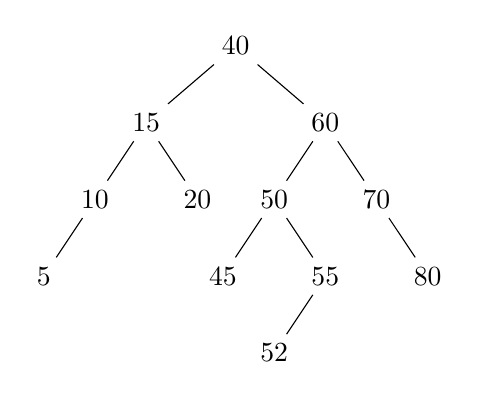
\begin{tikzpicture}[ level distance=1.5cm,
        level 1/.style={sibling distance=3.5cm},
        level 2/.style={sibling distance=2cm}, scale=.65]
            \node {40}
                child{node{15}
                        child{node{10} child{node{5}} child{node{} edge from parent
            [draw=none]}}
                        child{node{20}}}
                child{node{60}
                        child{node{50}
                                child{node{45}}
                                child{node{55}
                                        child{node{52}}
                                        child{node{} edge from parent [draw=none]}
                                }
                                }
                        child{node{70} child{node{} edge from parent [draw=none]}
                                child{node{80}}}
            };
    \end{tikzpicture}
    \end{center}
\begin{remark} Go over the properties and calculate the tree's height. Make sure you understand the definitions!
\end{remark}

Last time, we saw some operations that can be performed on BSTs, and
proved correctness for some of them. These were: $Search(x), Min(T), Max(T), Pred(x), Succ(x),
Insert(x), Delete(x)$. All of these operations take $O(h(T))$ in the worst case.\\

The main two operations that may cause problems are $Insert$ and $Delete$, as
they change the tree's height (consider inserting $81,82,83,84$ to our
working example).
To address this problem, we introduce another field: for each node $v$, add a field of $h(v)$ = the height of the subtree whose root is $v$. This allows us to maintain the AVL property:
\begin{defbox}{AVL Tree.} An AVL tree is a balanced BST, such that for any node $x$, its left and right subtrees' height differs in no more than $1$. In other words:
        $$|h(left(x)) - h(right(x))|\leq 1$$
    \end{defbox}
    This field allows us to calculate the Balance Factor for each node in $O
    (1)$:
    \begin{defbox}{Balance Factor.} For each node $x\in T$, it's Balance Factor is defined 
    $$hd
    (x) := h(left(x)) - h(right(x))$$ In AVL trees, we would like to maintain
    $|hd(x)| \leq 1$
    \end{defbox}
\begin{example} For our working example, the node $60$'s $hd$ is $h(50) - h
(70) = 1$, and $hd(50) = h(45)- h(55) = -1$. You can check and see that this is an AVL tree.
\end{example}
So to make sure that we can actually maintain time complexity $O(\log(n))$, we would want to:
\begin{enumerate}
    \item Show that for an AVL tree, $h(T) = \theta(log(n))$ (If there's time
    left)
    \item See how to correct violations in AVL property - using \textbf{rotations}
    \item See how to $Delete$ and $Insert$, while maintaining the height field.
\end{enumerate}

%\newpage
\subsection{Rotations}
\begin{figure}[h]
  \centering
\includegraphics[scale=.3]{Recitations/rotations.png}\\
\end{figure}
Rotations allow us to maintain the AVL property in $O(1)$ time (you have
discussed this in the lecture - changing subtree's roots).
In
this
schematic
representation of rotations, $x,y$ are nodes and $\alpha,\beta,\gamma$ are subtrees.
Note that the BST property is maintained! \\

%\includegraphics[scale=.5]{Recitations/rotationEg.png}

The Balance factor allows us to identify if the AVL property was violated, and moreover -
the exact values of the bad Balance factors will tell us which rotations to do to fix
this:\\
Taken from last year's recitation:\\
\includegraphics[scale=.6]{Recitations/violations.png}

Let us analyze one of these cases:\\
\begin{example} Let us see why R rotation Fixes LL violation:\\
\begin{figure}[h]
  \centering
\includegraphics[scale=.5]{Recitations/LLviolation.jpg}\\
This is the general form of LL violations.
\end{figure}

Let us analyze the heights of subtrees. Denote $h$ the height of $A_L$ before inserting $v$. So $A_R$'s height has also to be $h$.
If its height were $h+1$, the insertion would not have created a violation in
$B$ ($A$'s height would have stayed the same). If it were $h-1$, the violation would have appeared first in $A$ (not in $B$). Thus, $A$'s height is $h+1$.
$B_R$'s height is also $h$: If it was $h+1$ or $h+2$, no violation in $B$ had
occurred.

After the rotation, the tree looks like this:
\begin{figure}[h]
  \centering
  \includegraphics[scale=.9]{Recitations/LLviolationfix.jpg}
\end{figure}
So all the nodes here maintain AVL property; why is it maintained?
\end{example}\\
Detect the violation in the following tree, and perform the necessary rotations:\\
\begin{figure}[h]
  \centering
  \begin{subfigure}[b]{0.31\textwidth}
            \begin{tikzpicture}[ level distance=1.5cm,
        level 1/.style={sibling distance=3.5cm},
        level 2/.style={sibling distance=2cm}, scale=.65]
            \node {15}
	    child{node{5} child{node{3}} child{node{12}  child{node{10}
            child{node{6}} child{node{} edge from parent [draw = none]}}
            child{node{13}}}} child{node{20} child{node{18}} child{node{23}}}
            ;
    \end{tikzpicture}
  \end{subfigure}
\begin{subfigure}[b]{0.31\textwidth}
        \begin{tikzpicture}[ level distance=1.5cm,
        level 1/.style={sibling distance=3.5cm},
        level 2/.style={sibling distance=2cm}, scale=.65]
            \node {15}
	    child{node{} child{node{3}} child{node{10}
            child{node{6}} child{node{12} child{node{} edge
            from parent [draw = none]} child{node{13}} }}
            }
             child{node{20} child{node{18}} child{node{23}}}
            ;
    \end{tikzpicture}
  \end{subfigure}
\begin{subfigure}[b]{0.31\textwidth}
  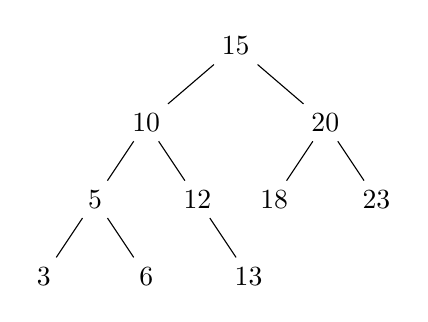
\begin{tikzpicture}[ level distance=1.5cm,
        level 1/.style={sibling distance=3.5cm},
        level 2/.style={sibling distance=2cm}, scale=.65]
            \node {15}
                child{node{10} child{node{5} child{node{3}} child{node{6}}
            } child{node{12}
            child{node{} edge from parent [draw = none]} child{node{13}}}}
             child{node{20} child{node{18}} child{node{23}}}
            ;
    \end{tikzpicture}

\end{subfigure}
  \caption{ 
The first node in which a violation occurred is $5$, this is an RL violation.
Perform R rotation on the right child. Then perform L rotation on the root of the relevant subtree ($5$):
}
\end{figure}
\subsection{Delete, Insert.}
The principles of the $Delete$ and $Insert$ operations are the same as in
regular BST, but we will need to rebalance the tree in order to preserve AVL
property.
A single insertion or deletion may change the height difference of subtrees
by at most 1, and might affect only the subtrees with roots along the path
from $r$ to the point of insertion/ deletion.
More concretely - we will add a recursive operation of traversing the tree
"back up" and checking violations. Had we found one - we will fix it using
rotations. Since rotations can be done in $O(1)$, the entire correction
process will take $O(\log(n))$, so we maintain a good time complexity.


{AVL Insert(r,x)}
  \begin{algorithm}[H]
    Call Insert $(r,x)$ // (The standard insertion routine for BST) \\  
    Let $p$ be the new node appended to the tree. \\
    \While{ $p$.parent $\neq \emptyset $ } {
      Check which of the four states we are in.\\ 
      Apply the right rotation. \\ 
      Update the height of each touched vertex  \\
      $p \leftarrow$ $p$.parent \\  
    }
  \end{algorithm}



\iffalse
\newpage
\subsection{Delete, Insert}
The principles of the $Delete$ and $Insert$ operations are the same as in
regular BST, but we will need to rebalance the tree in order to preserve AVL
property.
A single insertion or deletion may change the height difference of subtrees
by at most 1, and might affect only the subtrees with roots along the path
from $r$ to the point of insertion/ deletion.
More concretely - we will add a recursive operation of traversing the tree
"back up" and checking violations. Had we found one - we will fix it using
rotations. Since rotations can be done in $O(1)$, the entire correction
process will take $O(\log(n))$, so we maintain a good time complexity.
\subsubsection{Delete}
This is the regular BST delete. We will need to traverse up the
tree and detect violations (if occurred).\\
\includegraphics[scale=.6]{Recitations/DeleteBST.jpg}\\
\begin{remark} Go over the procedure quickly - explain the 3 cases - no
children, one child (easy), and two children (using successor).
\end{remark}
\begin{example}\\
    Delete $20$ from the tree at the beginning of the recitation:\\
    \includegraphics[scale=.3]{Recitations/DeleteEx.jpg}
\end{example}
%    Consider the original BST we looked at:\\
%
%\begin{tikzpicture}[ level distance=1.5cm,
%        level 1/.style={sibling distance=3.5cm},
%        level 2/.style={sibling distance=2cm}, scale=.65]
%            \node {40}
%                child{node{15}
%                        child{node{10} child{node{5}} child{node{} edge from parent
%            [draw=none]}}
%                        child{node{20}}}
%                child{node{60}
%                        child{node{50}
%                                child{node{45}}
%                                child{node{55}
%                                        child{node{52}}
%                                        child{node{} edge from parent [draw=none]}
%                                }
%                                }
%                        child{node{70} child{node{} edge from parent [draw=none]}
%                                child{node{80}}}
%            };
%    \end{tikzpicture}
%
%Let's $Insert(4)$:\\
%
%\begin{tikzpicture}[ level distance=1.5cm,
%        level 1/.style={sibling distance=3.5cm},
%        level 2/.style={sibling distance=2cm}, scale=.65]
%            \node {40}
%                child{node{15}
%                        child{node{(-2)10} child{node{(-1)5}child{node{4}}
%            child{node{} edge
%            from
%            parent
%            [draw = none]} }
%            child{node{} edge from
%            parent
%            [draw=none]}}
%                        child{node{20}}}
%                child{node{60}
%                        child{node{50}
%                                child{node{45}}
%                                child{node{55}
%                                        child{node{52}}
%                                        child{node{} edge from parent [draw=none]}
%                                }
%                                }
%                        child{node{70} child{node{} edge from parent [draw=none]}
%                                child{node{80}}}
%            };
%    \end{tikzpicture}\\
%
%So we need to fix LL violation. This is by performing R rotation of the root
%of the subtree in which the violation first appeared: \\
%
%\begin{tikzpicture}[ level distance=1.5cm,
%        level 1/.style={sibling distance=3.5cm},
%        level 2/.style={sibling distance=2cm}, scale=.65]
%            \node {40}
%                child{node{15}
%                        child{node{(0)5} child{node{(0)4}} child{node{10}}
%             }
%                        child{node{20}}}
%                child{node{60}
%                        child{node{50}
%                                child{node{45}}
%                                child{node{55}
%                                        child{node{52}}
%                                        child{node{} edge from parent [draw=none]}
%                                }
%                                }
%                        child{node{70} child{node{} edge from parent [draw=none]}
%                                child{node{80}}}
%            };
%    \end{tikzpicture}
%\begin{remark}
%    RR rotations are symmetric
%\end{remark}
\subsubsection{Insert}
Once again - this is the regular BST insert; we will need to traverse up the
tree and detect violations (if occurred).\\
\includegraphics[scale=.6]{Recitations/InsertBST.jpg}\\
\begin{example}
    Insert $65$ tho the previous tree (after the deletion):\\
    \begin{tikzpicture}[ level distance=1.5cm,
        level 1/.style={sibling distance=3.5cm},
        level 2/.style={sibling distance=2cm}, scale=.65]
            \node{50} child{node{40} child{node{10} child{node{5}
            }child{node{15}}} child{node{45}}}
            child{node{60} child{node{55}
                                    child{node{52}} child{node{} edge from
                                                            parent [draw=none]}}
                                    child{node{70}
                                            child{node{} edge from parent
            [draw=none]} child{node{80}}}}

    \end{tikzpicture}\\
    So after the insertion:\\
        \begin{tikzpicture}[ level distance=1.5cm,
        level 1/.style={sibling distance=3.5cm},
        level 2/.style={sibling distance=2cm}, scale=.65]
            \node{50} child{node{40} child{node{10} child{node{5}
            }child{node{15}}} child{node{45}}}
            child{node{60} child{node{55}
                                    child{node{52}} child{node{} edge from
                                                            parent [draw=none]}}
                                    child{node{70}
                                            child{node{65}} child{node{80}}}}

    \end{tikzpicture}\\
    And no violation occurred.\\
    \newpage
\end{example}
\begin{example}
    Insert 53 to the previous tree:\\
    \begin{tikzpicture}[ level distance=1.5cm,
        level 1/.style={sibling distance=3.5cm},
        level 2/.style={sibling distance=2cm}, scale=.65]
            \node{50} child{node{40} child{node{10} child{node{5}
            }child{node{15}}} child{node{45}}}
            child{node{60} child{node{55}
                                    child{node{52} child{node{} edge from
            parent [draw=none]} child{node{53}}} child{node{}
            edge
            from
                                                            parent [draw=none]}}
                                    child{node{70}
                                            child{node{65}} child{node{80}}}}

    \end{tikzpicture}\\
    Detect LR violation in $55$: Perform $L$ rotation on $52$:\\
    \begin{tikzpicture}[ level distance=1.5cm,
        level 1/.style={sibling distance=3.5cm},
        level 2/.style={sibling distance=2cm}, scale=.65]
            \node{50} child{node{40} child{node{10} child{node{5}
            }child{node{15}}} child{node{45}}}
            child{node{60} child{node{55}
                                    child{node{53} child{node{52}}
            child{node{} edge from parent[draw=none]}}
            child{node{}
            edge
            from
                                                            parent [draw=none]}}
                                    child{node{70}
                                            child{node{65}} child{node{80}}}}

    \end{tikzpicture}\\
    perform $R$ rotation on $55$:\\
    \begin{tikzpicture}[ level distance=1.5cm,
        level 2/.style={sibling distance=3cm},
        level 1/.style={sibling distance=5cm},
        level 3/.style={sibling distance=1.5cm},scale=.65]
            \node{50} child{node{40} child{node{10} child{node{5}
            }child{node{15}}} child{node{45}}}
            child{node{60} child{node{53}
                                    child{node{52}}
            child{node{55}}}
                                    child{node{70}
                                            child{node{65}} child{node{80}}}}

    \end{tikzpicture}\\

\end{example}

\newpage
\fi
\subsection{Exam Question.}
Consider the following question from 2018 exam. 
\begin{figure}[h]
  \centering
  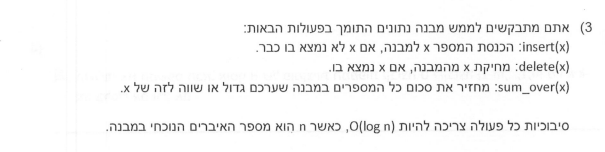
\includegraphics[scale=0.8]{avl-q-exam.png}\\
\end{figure}



\begin{figure}[H]
  \begin{subfigure}[b]{0.47\textwidth}
    \paragraph{Solution.} 

How would it look like an algorithm which computes the 'sum over' query? Or for given $x$, which vertices have a key less than $x$? 
Consider the path $v_1,v_2,v_3...v_n$ on which the Search subroutine went over when looking for $x$. If $v_i$.key $ <  v_{i+1}$.key then it means that $x$ is 
greater then $v_{i}$.key. Furthermore, $x$ is also greater than all the keys in the left subtree of $v_{i}$.

\paragraph{}

Let us transform that insight into an 
Algorithm. Define for each vertex a field that stores the summation of all its left subtree keys plus its own key; call it 'Leftsum'.  
Then computing the sumover query will be done by summing these fields of the vertices in the right turn on the searching path. 
\end{subfigure} 
\hfill
\begin{subfigure}[b]{0.49\textwidth}
  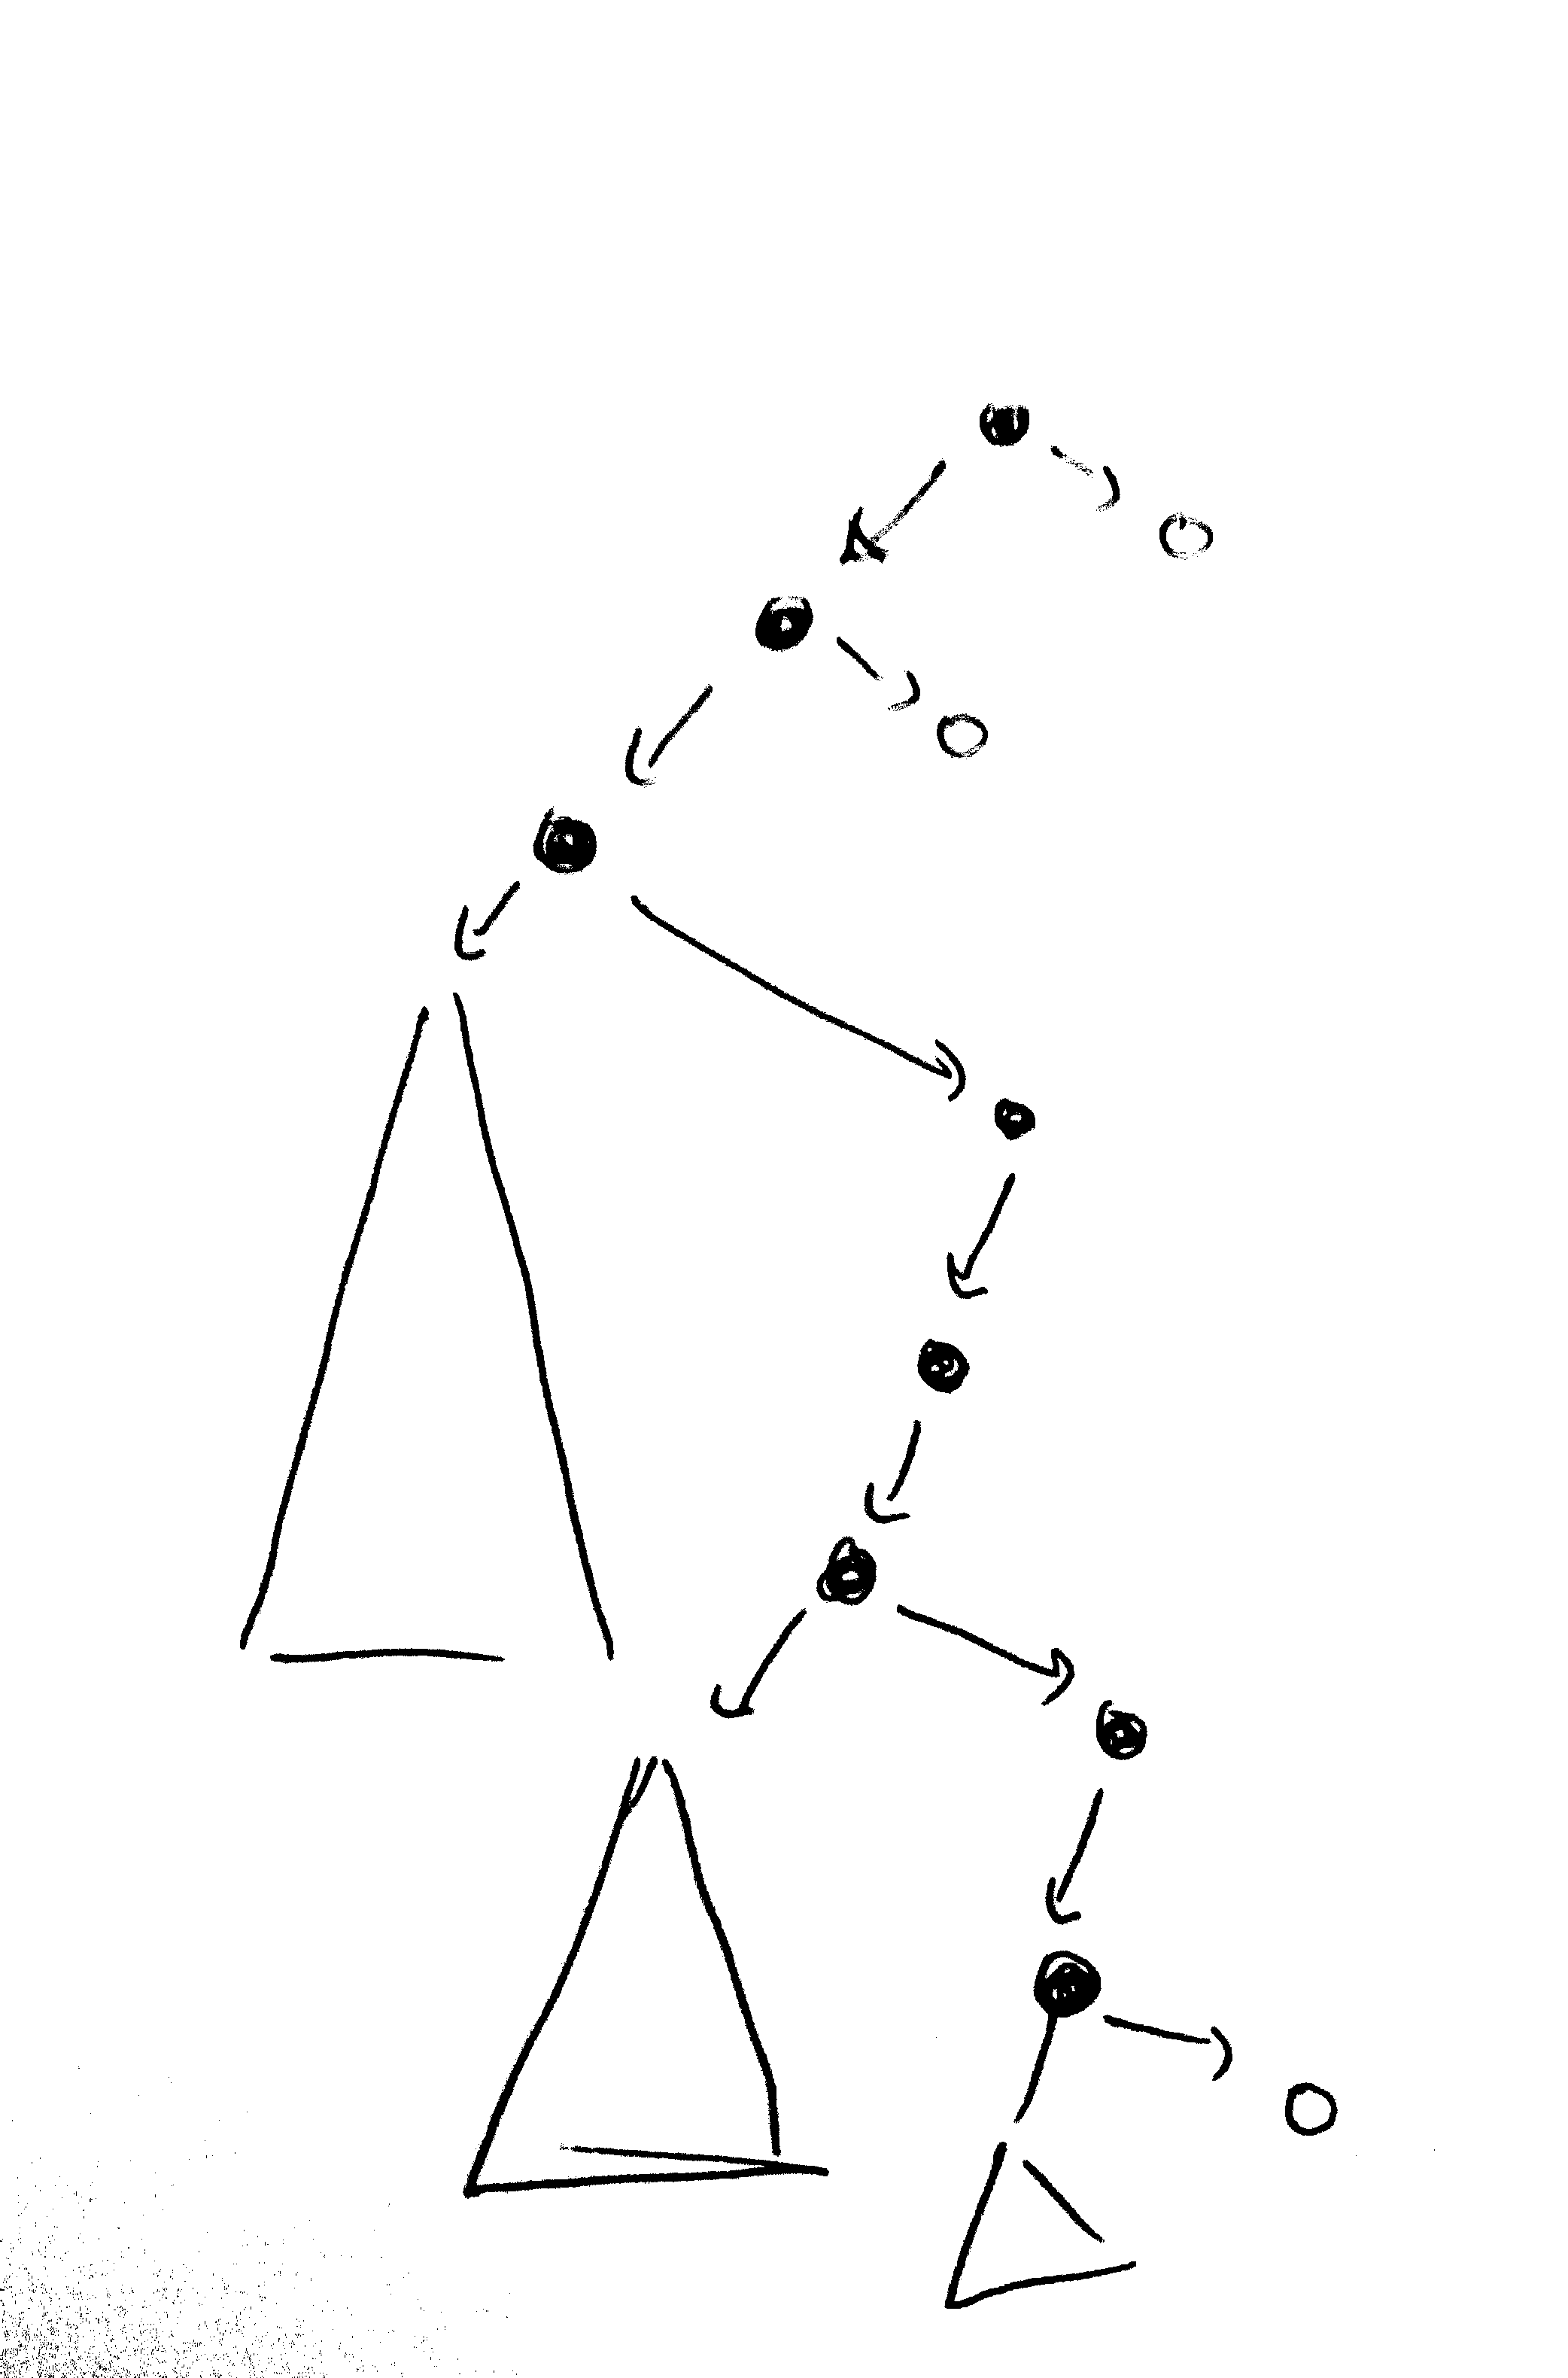
\includegraphics[scale=0.07]{oavl-q.png}
   \end{subfigure} 
   \hfill
\end{figure}


{Sumover($r$,$x$)}
  \begin{algorithm}[H]
    \If{ $r$ is None }{
      return $0$ 
    }\Else{
      \If{$x > r$.key }{
	return $r$.Leftsum + Sumover( $r$.right, $x$ )  
      }\Else{
      	return Sumover( $r$.left, $x$ )  
      }
    }
  \end{algorithm}


So it has left to show how one could maintain the tree and guarantee a logarithmic height. Consider a vertex $v$ and suppose that both
his direct children are correct AVL trees and have the correct value at the Leftsum field. We know that:
\begin{enumerate}
  \item There is a rotation that balances the tree at the cost of $O(1)$ time.
  \item All the descendants of $v$, at a distance at least two from it,  will remain the same in the sense that their subtree has not changed. 
\end{enumerate}
Therefore we will have to recompute the Sumleft filed for only a $O(1)$ vertices (which are the children and the grandchildren of $v$ previews the rotation). 
Each computation could be done in $O(1)$ time. 


{AVL-Leftsum Insert(r,x)}
  \begin{algorithm}[H]
    Call Insert $(r,x)$ // (The standard insertion routine for BST) \\  
    Let $p$ be the new node appended to the tree. \\
    \While{ $p$.parent $\neq \emptyset $ } {
      Apply the right rotation. \\
      \For{ any vertex $v$ such that its pointers have changed, sorted by height } {
	$v$.Leftsum $\leftarrow$ $v$.key + $v$.left.Leftsum + $v$.left.right.Leftism 		
      }
      $p \leftarrow$ $p$.parent \\  
    }
  \end{algorithm}


\paragraph{Running time.} The work is done over vertices along a single path, and on each vertex only $O(1)$ time 
is spent, Then we have that the total running time of the algorithm is proportional to the tree height. 
Combining the fact that we maintain the AVL property, it follows that the total time is $\Theta\left( \log n \right)$.  




\section*{Appendix}
\subsection{AVL tree's height}
Let $n_h$ be the minimal number of nodes in an AVL tree of height
$h$.\\
\begin{thm}
    $n_h$ is strictly increasing in $h$.
\end{thm}
\begin{proof} Exercise.
\end{proof}
\begin{thm}
$n_{h} = n_{h-1} + n_{h-2} + 1$.
\end{thm}
\begin{proof}For an AVL tree of height $0$, $n_0 = 1$,
and of height $1$, $n_1 = 2 $ (by checking directly).\\
    Let's look at a minimal AVL tree of height $h$. By the AVL property, one
of its subtrees is of height $h-1$ (WLOG - the left subtree) and by
minimality, its left subtree has to have $n_{h-1}$ nodes. $T$'s right subtree
thus has to be of height $h-2$: It can't be of height $h-1$: $n_{h-1} >
n_{h-2}$ by the previous theorem, and if the right subtree is of height $h-1$ -
we could switch it with an AVL tree of height $h-2$, with fewer nodes - so
less nodes in $T$, contradicting minimality. So the right subtree has
$n_{h-2}$ nodes (once again, by minimality), and thus the whole tree has
    $n_{h} = n_{h-1} + n_{h-2} + 1$ (added the root) nodes.
\end{proof}
\begin{cor}$n_h > 2n_{h-2} + 1$
\end{cor}
\begin{cor}$h = O(\log(n))$
\end{cor}
\begin{proof}
    Assume $k$ is even (why can we assume that?).
    It can be shown by induction that:
    \[
        n_h>2n_{h-2}+1>2(2n_{h-4}+1)+1=4n_{h-4}+(1+2)\ldots >
        2^{\frac{h}{2}}+\sum_{i=0}^{\frac{h}{2}-1}
        2^i=\sum_{i=1}^{\frac{h}{2}}2^i = \frac{2^\frac{h}{2} - 1}{2-1} =  2^{\frac{h}{2}} - 1
    \]
    So $n_h \geq 2^{\frac{h}{2}} - 1$, thus
    \[
        h\leq 2\log(n_h + 1)
    \]
    and for generall AVL tree with $n$ nodes and height $h$:
    \[
         h\leq 2\log(n_h + 1) \leq 2\log(n + 1) = O(\log(n))
    \]
%    By $n_h$'s minimality:
%    $$n \geq n_h \geq F_h = C (\varphi^h - (-\varphi)^h) \geq
%    \tilde{C}\varphi^h$$
%    Thus
%    $h \leq \frac{1}{\tilde{C}} \log_{\varphi}(n)$
\end{proof}
\begin{remark}
    In fact, one can show that $n_h > F_h$ and $F_h$ is the $h$'th Fibonacci
    number. Recall that $F_h = C(\varphi^h - (\psi)^h)$, and this gives a
    tighter bound on $n_h$.
\end{remark}

\newpage\chapter{Graphs  - Recitation 9} 

\usetikzlibrary{positioning, arrows}
\tikzset{main node/.style={circle,draw,minimum size=0.8cm,inner sep=0pt},}
\tikzset{edge/.style = {->,> = latex'}}

\iffalse
\newtheorem{prop}{Proposition}
\newtheorem{ex}{Exercise}
\newtheorem{sol}{Solution}
\newtheorem{theorem}{Theorem} \newtheorem{thm}{Theorem}[section]
\newtheorem{conj}[thm]{Conjecture} \newtheorem{lemma}[thm]{Lemma}
\newtheorem{corollary}[thm]{Corollary} \newtheorem{claim}[thm]{Claim}
\newtheorem{proposition}[thm]{Proposition}
\newtheorem{definition}{Definition} \newtheorem{remark}{Remark}
   
\pagestyle{empty}

\setlength{\textwidth}{6.5in}
\setlength{\evensidemargin}{0.0in}
\setlength{\oddsidemargin}{0.0in}
\setlength{\topmargin}{-0.25in}
\setlength{\textheight}{9.0in}
\setlength{\baselineskip}{1.3\baselineskip}
\setlength{\parindent}{.0in}
\fi
\tikzset{
node of list/.style = { 
             draw, 
             fill=orange!20, 
             minimum height=6mm, 
             minimum width=6mm,
             node distance=6mm
   },
link/.style = {
     -stealth,
     shorten >=1pt
     },
array element/.style = {
    draw, fill=white,
    minimum width = 6mm,
    minimum height = 10mm
  }
}

\def\LinkedList#1{%
  \foreach \element in \list {
     \node[node of list, right = of aux, name=ele] {\element};
     \draw[link] (aux) -- (ele);
     \coordinate (aux) at (ele.east);
  } 
}



%%%%%%%%%%%%%%%%%%%%%%%%%%%%%%%%%%%%%%%%%%%%%%%%%%%%%%%%%%%%



%%%%%%%%%%%%%%%%%%%%%%%%%%%%%%%%%%%%%%%%%%%%%%%%%%%%%%%%%%%%

%\vspace{0.2in}

\section{Graphs}
This is an important section, as you'll see graphs A LOT in this course and in the courses to follow. 

\subsection{Definitions, Examples, and Basics}

\begin{figure}[h]
\begin{subfigure}[b]{0.65\textwidth}
\begin{definition}
A \textbf{non-directed graph} $G$ is a pair of two sets - $G=(V, E)$ - $V$ being a set of vertices and $E$ being a set of couples of vertices, which represent edges ("links") between vertices.
\end{definition}

\textbf{Example}: $G= (\{1,2,3,4\},\ \{\{1,2\}, \{1,3\}, \{3,4\}\})$ is the following graph:\\ 
\end{subfigure}
\begin{subfigure}[b]{0.05\textwidth}
  \
\end{subfigure}
  \begin{subfigure}[b]{0.25\textwidth}
    \begin{tikzpicture}
\node[main node](1){$1$};
\node[main node](2)[below = 1cm of 1]{$2$};
\node[main node](3)[right = 1cm of 1]{$3$};
\node[main node](4)[below = 1cm of 3]{$4$};

\path[draw, thick]
(1) edge node {} (2)
(1) edge node {} (3)
(3) edge node {} (4);
\end{tikzpicture}
\end{subfigure}
\end{figure}
\begin{figure}[h]
\begin{subfigure}[b]{0.65\textwidth}
\begin{definition}
A \textbf{directed graph} $G$ is a pair of two sets - $G=(V, E)$ - $V$ being a set of vertices and $E\subseteq V\times V$ being a set of directed edges ("arrows") between vertices.
\end{definition}
\textbf{Example}: $G=(\{1,2,3,4\},\ \{(1, 2), (1, 4), (4, 1), (4,3)\})$ is the following graph (note that it has arrows): \\ 
\end{subfigure}
\begin{subfigure}[b]{0.05\textwidth}
  \
\end{subfigure}
  \begin{subfigure}[b]{0.25\textwidth}
    \begin{tikzpicture}
\node[main node](1){$1$};
\node[main node](2)[below = 1cm of 1]{$2$};
\node[main node](3)[right = 1cm of 1]{$3$};
\node[main node](4)[below = 1cm of 3]{$4$};

\draw[edge] (1) to (2);
\draw[edge] (1) to (4);
\draw[edge] (4) to (1);
\draw[edge] (4) to (3);
\end{tikzpicture}
\end{subfigure}
\end{figure}

\begin{definition}
  A \textbf{weighted graph} composed by a graph $G=\left( V,E \right)$ (either non-directed or directed) and a weight function $w : E \rightarrow \mathbb{R}$. Usually (but not necessary), we will think about the quantity $w(e)$, where $e \in E$, as the length of the edge.  
\end{definition}

Now that we see graphs with our eyes, we can imagine all sorts of uses for them... For example, they can represent the structure of the connections between friends on Facebook, or they can even represent which rooms in your house have doors between them.

\begin{remark}
Note that directed graphs are a \textbf{generalization} of non-directed graphs, in the sense that every non-directed graph can be represented as a directed graph. Simply take every non-directed edge $\{v,u\}$ and turn it into two directed edges $(v,u), (u,v)$. 
\end{remark}

\begin{remark}
Note that most of the data structures we discussed so far - Stack, Queue, Heap, BST - can all be implemented using graphs.
\end{remark}

Now let's define some things in graphs:

\begin{definition} (Path, circle, degree)
\begin{enumerate} 
\item A \textbf{simple path} in the graph $G$ is a series of unique vertices (that is, no vertex appears twice in the series) $v_1, v_2, ..., v_n$ that are connected with edges in that order. 
\item A \textbf{simple circle} in the graph $G$ is a simple path such that $v_1 = v_n$. 
\item The \textbf{distance} between two vertices $v,u\in V$ is the length of the shortest path between them ($\infty$ if there is no such path).
\end{enumerate}
\end{definition}

\begin{remark}
Note that for all $u,v,w\in V$ the triangle inequality holds regarding path lengths. That is:
$$dist(u,w)\leq dist(u,v) + dist(v, w)$$
\end{remark}

\begin{definition} (connectivity)
\begin{enumerate}
  \item Let $ G =\left( V,E \right)$ be a non-directed graph. A \textbf{connected component} of $G$ is a subset $U \subseteq V$ of maximal size in which there exists a path between every two vertices. 
\item A non-directed graph $G$ is said to be a \textbf{connected} graph if it only has one connected component.
\item Let $ G = \left(V, E\right)$ be a directed graph. A \textbf{strongly connected component} of $G$ is a subset $U \subseteq V$ of maximal size in which for any pair of vertices $u,v \in U$ there exist both directed path from $u$ to $v$ and a directed path form $v$ to $u$.   
\end{enumerate}
\end{definition}
%\begin{figure}[h]
  %\begin{subfigure}[b]{0.4\textwidth} 
%An \textbf{example} of a non-connected graph: \\ \\ \\  \\
%\end{subfigure}
%\begin{subfigure}[b]{0.05\textwidth}
  %\
%\end{subfigure}
%\begin{subfigure}[b]{0.25\textwidth}
%\begin{tikzpicture}
%\node[main node](1){$1$};
%\node[main node](2)[below = 1cm of 1]{$2$};
%\node[main node](3)[right = 1cm of 1]{$3$};
%\node[main node](4)[below = 1cm of 3]{$4$};
%
%\draw[edge] (1) to (2);
%\draw[edge] (3) to (4);
%\end{tikzpicture}
%\end{subfigure}
%\end{figure}

\begin{prop}
Let $G=(V,E)$ be some graph. If $G$ is connected, then $|E| \geq |V|-1$
\end{prop}

\begin{proof}
We will perform the following cool process: Let $\{e_1,...,e_m\}$ be an enumeration of $E$, and let $G_0=(V,\emptyset)$. We will build the graphs $G_1, G_2,... G_m=G$ by adding edges one by one. Formally, we define - 
$$\forall i\in[m]\ \ G_i=(V,\{e_1,...,e_i\})$$
$G_0$ has exactly $|V|$ connected components, as it has no edges at all. Then $G_1$ has $|V|-1$. From there on, any edges do one of the following:
\begin{enumerate}
    \item Keeps the number of connected components the same (the edge closes a cycle)
    '\item Lowers the number of connected components by $1$ (the edges does not close a cycle)
\end{enumerate}

So in general, the number of connected components of $G_i$ is $\geq |V|-i$. 
Now, if $G_m=G$ is connected, it has just one connected component! This means:
$$1 \geq |V| - |E|\ \implies \ |E|\geq|V|-1$$

\end{proof}


\subsection{Graph Representation}

Okay, so now we know what graphs are. But how can we represent them in a computer? There are two main options. The first one is by \textbf{array of adjacency lists}. Given some graph $G$, every slot in the array will contain a linked list. Each linked list will represent a list of some node's neighbors. The second option is to store edges in an \textbf{adjacency matrix}, a $ |V| \times |V| $ binary matrix in which the $v,u$-cell equals $1$ if there is an edge connecting $u$ to $v$. That matrix is denoted by $A_{G}$ in the example below. Note that the running time analysis might depend on the underline representation.     

\textbf{Question.} What is the memory cost of each of the representations? Note that while holding an adjacency matrix requires storing $|V|^2$ bits regardless of the size of $E$, Maintaining the edges by adjacency lists costs linear memory at the number of edges and, therefore, only $ \Theta \left(  |V| + |E| \right) $ bits. 

\paragraph{Example.} Consider the following directed graph:
\begin{figure}[h]
  \centering
  \begin{subfigure}[b]{0.25\textwidth}
    \begin{tikzpicture}
      \node[main node](1){$1$};
      \node[main node](2)[below = 1cm of 1]{$2$};
      \node[main node](3)[right = 1cm of 1]{$3$};
      \node[main node](4)[below = 1cm of 3]{$4$};

      \draw[edge] (1) to (2);
      \draw[edge] (1) to (4);
      \draw[edge] (4) to (1);
      \draw[edge] (4) to (3);
      \draw[edge] (1) to (3);
      \draw[edge] (3) to (1);
    \end{tikzpicture}  
    \\ \\  
  \end{subfigure} 
  \begin{subfigure}[b]{0.49\textwidth}
    \begin{tikzpicture}
      \foreach \index/\list in {1/{2,3,4,null}, 2/{null}, 3/{1, null}, 4/{1, 3, null}} {
	\node[array element] (aux) at (0,-\index) {\index};
	\LinkedList{\list}
      }
    \end{tikzpicture}  
  \end{subfigure}
  \caption{ Persenting $G$ by array of adjacency lists.  }
\end{figure}

%Its representation will be: \\ \\

\begin{figure}[h]
  \centering
  \begin{subfigure}[b]{0.25\textwidth}
        \begin{tikzpicture}
\node[main node](1){$1$};
\node[main node](2)[below = 1cm of 1]{$2$};
\node[main node](3)[right = 1cm of 1]{$3$};
\node[main node](4)[below = 1cm of 3]{$4$};

\draw[edge] (1) to (2);
\draw[edge] (1) to (4);
\draw[edge] (4) to (1);
\draw[edge] (4) to (3);
\draw[edge] (1) to (3);
\draw[edge] (3) to (1);
\end{tikzpicture} \\ 
  \end{subfigure}
\begin{subfigure}[b]{0.49\textwidth}       
  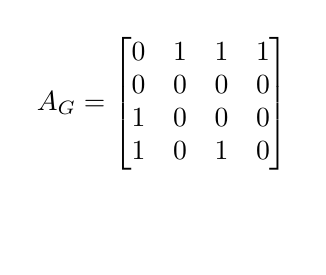
\begin{tikzpicture}
    \node (1) at (0,0) { };
    \node  (2) at (1,1.7) { $ A_{G} = 
	  \begin{bmatrix}
	0 & 1 & 1 & 1\\
	0 & 0 & 0 & 0\\
	1 & 0 & 0 & 0\\
	1 & 0 & 1 & 0
	\end{bmatrix}
      $ };
      \end{tikzpicture}
\end{subfigure}
\caption{ Presenting $G$ by adjacency matrix. }
\end{figure}

\subsection{Breadth First Search (BFS)}

One natural thing we might want to do is to travel around inside a graph. That is, we would like to visit all of the vertices in a graph in some order that relates to the edges. 
Breadth-first search constructs a breadth-first tree, initially containing only its root, which is the source vertex $s$. Whenever the search discovers a white vertex $v$ in the course of scanning the adjacency list of a gray vertex $u$, the vertex $v$ and the edge ($u$, $v$) are added to the tree. We say that $u$ is the predecessor or parent of $v$ in the breadth-first tree. Since every vertex reachable from $s$ is discovered at most once, each vertex reachable from $s$ has exactly one parent. (There is one exception: because $s$ is the root of the breadth-first tree, it has no parent.) Ancestor and descendant relationships in the breadth-first tree are defined relative to the root $s$ as usual: if $u$ is on the simple path in the tree from the root $s$ to vertex $v$, then $u$ is an ancestor of $v$, and $v$ is a descendant of $u$.
The breadth-first-search procedure BFS on the following page assumes that the graph $G = (V, E)$ is represented using adjacency lists. It denotes the queue by $Q$, and it attaches three additional attributes to each vertex $v$ in the graph:

\begin{enumerate}
    \item $v$.visited is a boolean flag which indicate wheter $v$ was allready visited.
    \item $\pi(v)$ is $v$’s predecessor in the breadth-first tree. If $v$ has no predecessor because it is the source vertex or is undiscovered, then $\pi(v)$ is None/NULL.
\end{enumerate}

{BFS($G, s$)}
  \begin{algorithm}[H]
    \For {$v\in V$}{
	 $v.visited \leftarrow $ False 
     }
 $Q\leftarrow$ new Queue \\ 
 $Q$.Enqueue($s$) \\
 $s$.visited $\leftarrow$ True \\
 \While {$Q$ is not empty} {
 $u\leftarrow Q$.Dequeue() \\
	\For {neighbor $w$ of $u$} {
	\If {$w$.visited is False}{
		 $w$.visited$\leftarrow$ True \\
		 $\pi(w) \leftarrow u $ \\
		 $Q$.Enqueue($w$)

	      }
	}
      }
  \end{algorithm}


\underline{Correctness}: The example should be enough to explain the correctness. A concrete proof can be found in the book, page 597.

\underline{Runtime}: We can analyse the runtime line-by-line:
\begin{itemize}
\item Lines 1-2: $|V|$ operations, all in $O(1)$ runtime, for a total of $O(|V|)$.
\item Lines 3-6: $O(1)$
\item Lines 7-8: First we need to understand the number of times the $while$ loop iterates. We can see that every vertex can only enter the queue ONCE (since it is then tagged as "visited"), and therefore it runs $\leq |V|$ times. All operations are $O(1)$, and we get a total of $O(|V|)$. 
\item Lines 9-13: Next, we want to understand the number of times this $for$ loop iterates. 
The for loop starts iterating once per vertex, and then the number of its iterations is the same as the number of neighbors that this vertex has. Thus, it runs $O(|E|)$ times.
\end{itemize}
So all in all we get a runtime of $O(|V|+|E|)$

\subsection{Usage of BFS}
Now we have a way to travel through a graph using the edges. How else can we use it?\\ \\ 
\textbf{Exercise}: Present and analyse an algorithm $CC(G)$ which receives some undirected graph $G$ and outputs the number of connected components in $G$ in $O(|V|+|E|)$. \\

\textbf{Solution}: Consider the following algorithm: (Now read the algorithm, it may be in the next page because LaTeX is dumb...)
{CC($G$)}
  \begin{algorithm}[H]
     count $\leftarrow 0$\\
     \For {$v\in V$ }{
	\If {$v$.visited = False} {
	  count$\leftarrow$count$+1$ \\
	  BFS($G, v$)
	}
      }
	\Return count
  \end{algorithm}


\subsection{Depth First Search (DFS)}
As its name implies, depth-first search searches "deeper" in the graph whenever possible. Depth-first search explores edges out of the most recently discovered vertex $v$ that still has unexplored edges leaving it. Once all of $ v$'s edges have been explored, the search "backtracks" to explore edges leaving the vertex from which $v$ was discovered. This process continues until all vertices that are reachable from the original source vertex have been discovered. If any undiscovered vertices remain, then depth-first search selects one of them as a new source, repeating the search from that source. The algorithm repeats this entire process until it has discovered every vertex.

{DFS($G$)}
  \begin{algorithm}[H]
   \bf{DFS}( $G$): \\
    \For {$v\in V$}{
 	$vi$.visited $\leftarrow False$
    }
    time $ \leftarrow 1 $\\
    \For {$v\in V$}{
      \If { not $v$.visited } {
	$\pi \left( v \right)  \leftarrow $ null \\ 
	Explore( $G,v$ ) 
     } 
   }

  \end{algorithm}

  \begin{algorithm}[H]
    \bf{Explore}($G,v$): \\
     Previsit($v$)
    \For {$\left( v,u \right) \in E  $}{
      \If { not $u$.visited } {
	$ \pi \left( u \right) \leftarrow v $ \\ 
	Explore( $G, u$ ) 
      }
    }
    Postvisit($v$)
  \end{algorithm}
  \begin{algorithm}[H]
    \bf{Previsit}($v$): \\
    pre($v$) $\leftarrow $ time \\
    time $\leftarrow$ time $+1$
  \end{algorithm}
 \begin{algorithm}[H]
   \bf{Postvisit} ($v$): \\ 
    post($v$) $\leftarrow $ time \\
    time $\leftarrow$ time $+1$
  \end{algorithm}



\paragraph{Properties of depth-first search.} Depth-first search yields valuable information about the structure of a graph. Perhaps the most basic property of depth-first search is that the predecessor subgraph $G_{\pi}$ does indeed form a forest of trees since the structure of the depth-first trees exactly mirrors the structure of recursive calls of explore-function. That is, $u$ = $\pi\left( v \right)$ if and only if explore($G, v$) was called during a search of $ u$'s adjacency list. Additionally, vertex $v$ is a descendant of vertex $u$ in the depth-first forest if and only if $v$ is discovered during the time in which $u$ is gray.
Another important property of depth-first search is that discovery and finish times have a parenthesis structure. If the explore procedure were to print a left parenthesis "$(u$" when it discovers vertex $u$ and to print a right parenthesis r``$u)$" when it finishes $u$, then the printed expression would be well-formed in the sense that the parentheses are properly nested.

The following theorem provides another way to characterize the parenthesis structure.

\paragraph{Parenthesis theorem}
In any depth-first search of a (directed or undirected) graph $G = (V, E)$, for any two vertices $u$ and $v$, exactly one of the following three conditions holds:

\begin{enumerate}
  \item the intervals [pre($u$), post($u$)] and [pre($v$), post($v$)] are entirely disjoint, and neither $u$ nor $v$ is a descendant of the other in the depth-first forest.
  \item the interval [pre($u$), post($u$)] is contained entirely within the interval [pre($v$), post($v$)], and $u$ is a descendant of $v$ in a depth-first tree, or
  \item the interval [pre($v$), post($v$)] is contained entirely within the interval [pre($u$), post($u$)], and $v$ is a descendant of $u$ in a depth-first tree.
  \end{enumerate}

  \paragraph{Proof.} We begin with the case in which pre($u$) $<$ pre($v$). We consider two subcases, according to whether pre($v$) $<$ post($u$). The first subcase occurs when pre($v$) $<$ post($u$), so that $v$ was discovered while $u$ was still gray, which implies that $v$ is a descendant of $u$. Moreover, since $v$ was discovered after $u$, all of its outgoing edges are explored, and $v$ is finished before the search returns to and finishes $u$. In this case, therefore, the interval [pre($v$), post($v$)] is entirely contained within the interval [pre($u$), post($u$)]. In the other subcase, post($u$) $<$ pre($v$), and by defintion, pre($u$) $<$ post($u$) $<$ pre(v) $<$ post($v$), and thus the intervals [pre($u$), post($u$)] and [pre($v$), post($v$)] are disjoint. Because the intervals are disjoint, neither vertex was discovered while the other was gray, and so neither vertex is a descendant of the other.



\paragraph{  Corollary. Nesting of descendants' intervals.}
  Vertex $v$ is a proper descendant of vertex $u$ in the depth-first forest for a (directed or undirected) graph $G$ if and only if pre($u$) $<$ pre($v$) $<$ post($v$) $<$ post($u$).

  
  %%\paragraph{Problem. Two Chess Pieces.}
 %Moti has a tree with n nodes. He is willing to share it with you, which means you can operate on it.

%Initially, there are two chess pieces on the node 1 of the tree. In one step, you can choose any piece, and move it to the neighboring node. You are also given an integer $d$. You need to ensure that the distance between the two pieces doesn't ever exceed $d$.

%Each of these two pieces has a sequence of nodes which they need to pass in any order, and eventually, they have to return to the root. As a curious boy, he wants to know the minimum steps you need to take.

%\paragraph{Solution.} We can find that for any $d$-th ancestor of some $b_i$, the first piece must pass it some time. Otherwise, we will violate the distance limit. The second piece must pass the $d$-th ancestor of each $b_i$ as well. Then we can add the $d$-th ancestor of each $a_i$ to the array $b$, and add the $d$-th ancestor of each $b_i$ to the array $a$.
%
%Then we can find now we can find a solution that each piece only needs to visit its nodes using the shortest route, without considering the limit of $d$, and the total length can be easily computed. We can find that if we adopt the strategy that we visit these nodes according to their DFS order(we merge the array of $a$ and $b$, and sort them according to the DFS order, if the first one is from $a$, we try to move the first piece to this position, otherwise use the second piece), and move the other piece one step closer to the present piece only if the next step of the present piece will violate the distance limit, then we can ensure the movement exactly just let each piece visit its necessary node without extra operations.
%


\newpage\chapter{Union Find - Recitation 11} 

\usetikzlibrary{positioning, arrows}
\tikzset{main node/.style={circle,draw,minimum size=0.8cm,inner sep=0pt},}
\tikzset{edge/.style = {->,> = latex'}}

\iffalse
  \newtheorem{prop}{Proposition}
  \newtheorem{ex}{Exercise}
  \newtheorem{sol}{Solution}
  \newtheorem{theorem}{Theorem} \newtheorem{thm}{Theorem}[section]
  \newtheorem{conj}[thm]{Conjecture} \newtheorem{lemma}[thm]{Lemma}
  \newtheorem{corollary}[thm]{Corollary} \newtheorem{claim}[thm]{Claim}
  \newtheorem{proposition}[thm]{Proposition}
  \newtheorem{definition}{Definition} \newtheorem{remark}{Remark}

  \pagestyle{empty}

  \setlength{\textwidth}{6.5in}
  \setlength{\evensidemargin}{0.0in}
  \setlength{\oddsidemargin}{0.0in}
  \setlength{\topmargin}{-0.25in}
  \setlength{\textheight}{9.0in}
  \setlength{\baselineskip}{1.3\baselineskip}
  \setlength{\parindent}{.0in}
\fi
\tikzset{
  node of list/.style = { 
    draw, 
    fill=orange!20, 
    minimum height=6mm, 
    minimum width=6mm,
    node distance=6mm
  },
  link/.style = {
    -stealth,
    shorten >=1pt
  },
  array element/.style = {
    draw, fill=white,
    minimum width = 6mm,
    minimum height = 10mm
  }
}

\def\LinkedList#1{%
  \foreach \element in \list {
    \node[node of list, right = of aux, name=ele] {\element};
    \draw[link] (aux) -- (ele);
    \coordinate (aux) at (ele.east);
  } 
}



%%%%%%%%%%%%%%%%%%%%%%%%%%%%%%%%%%%%%%%%%%%%%%%%%%%%%%%%%%%%



%%%%%%%%%%%%%%%%%%%%%%%%%%%%%%%%%%%%%%%%%%%%%%%%%%%%%%%%%%%%

%\vspace{0.2in}

\section{Union Find.} 

We have mentioned that to find efficiently the minimal spanning tree using Kruskal, One has to answer quickly about whether a pair of vertices $v,u$ share the same connectivity component. In this recitation, we will present a data structure that will allow us to query the belonging of a given item and merge groups at an efficient time cost. 

The problem defines as follows. Given $n$ items $x_1 ... x_{n}$, we would like to maintain the partition of them into disjoints sets by supporting the following operations:  
\begin{enumerate}
  \item Make-Set$(x)$ create an empty set whose only member is $x$. We could assume that this operation can be called over $x$ only once. 
  \item Union$(x,y)$ merge the set which contains $x$ with the one which contains $y$. 
  \item Find-Set$(x)$ returns a pointer to the set holding $x$. 
\end{enumerate}

Notice that the native implementation using pointers array, $A$, defined to store at place $i$ a pointer to the set containing $x$ can perform the Find-Set operation at $O\left( 1 \right)$. The bottleneck of that implementation is that the merging will require us to run over the whole items and changes their corresponding pointer at $A$ one by one. Namely, a running time cost of $\Theta\left( n \right)$ time. Let's review a diffrent approch:

\paragraph{Linked Lists Implementation.}
One way to have a non-trivial improvement is to associate each set with a linked list storing all the elements belonging to the set. Each node of those linked lists contains, in addition to its value and sibling pointer, a pointer for the list itself (the set). Consider the merging operation again. It's clear that having those lists allow us to unify sets by iterating and updating only the elements that belong to them. Still, one more trick is needed to achieve a good running cost. 


{Uinon$(x,y)$}
  \begin{algorithm}[H]
    \If{size $A[x] \ge $  size$A[y]$  }{
      size $A[x] \leftarrow $   size $A[x]$ +  size $A[y]$ \\
      \For{  $z \in A[y]$ }{
	$A[z] \leftarrow A[x]$ \\ 
      }
      $A[x] \leftarrow A[x] \cup A[y]$ // $O\left( 1 \right)$ concatenation of linked lists.  
    }\Else{
      Union $\left( y,x \right)$ 
    }
  \end{algorithm}


Executing the above over sets at linear size requires at least linear time. Let's analyze what happens when merging $n$ times. As we have seen in graphs, the runtime can be measured by counting the total number of operations each item/vertex does along the whole running. So we can ask ourselves how many times an item change its location and its set pointer. Assume that at the time when $x$ were changed $A[x]$ contains (before the merging) $t$ elements then immediately after that $A[x]$ will store at least $2t$ elements: 
\begin{equation*}
  \begin{split}
    \text{size } A^{(t+1)}[x] \leftarrow  \text{size } A^{(t)}[x] +  \text{size } A^{(t)}[y] \ge 2A^{(t)}[x]  
  \end{split}
\end{equation*}
Hence, if we list down the sizes of the $x$'s set at the moments merging occurred, we could write only $\log n$ numbers before exceeding the maximal size ($n$). That proves that the number of times the vertex changed his pointer is bounded by $\log n$, and the total number of actions costs at most $\Theta\left( n\log n \right)$. 

Notice that in the case in which $m = O\left( 1 \right)$, we will still pay much more than needed. Anyhow the next implementation is going to give us (eventually) a much faster algorithm.

%\begin{figure}[h]
  %\centering
  %\begin{subfigure}[b]{0.25\textwidth}
    %\begin{tikzpicture}
      %\node[main node](1){$1$};
      %\node[main node](2)[below = 1cm of 1]{$2$};
      %\node[main node](3)[right = 1cm of 1]{$3$};
      %\node[main node](4)[below = 1cm of 3]{$4$};
%
      %\draw[edge] (1) to (2);
      %\draw[edge] (1) to (4);
      %\draw[edge] (4) to (1);
      %\draw[edge] (4) to (3);
      %\draw[edge] (1) to (3);
      %\draw[edge] (3) to (1);
    %\end{tikzpicture}  
    %\\ \\  
  %\end{subfigure} 
  %\begin{subfigure}[b]{0.49\textwidth}
    %\begin{tikzpicture}
      %\foreach \index/\list in {1/{2,3,4,null}, 2/{null}, 3/{1, null}, 4/{1, 3, null}} {
	%\node[array element] (aux) at (0,-\index) {\index};
%	%\LinkedList{\list}
      %}
    %\end{tikzpicture}  
  %\end{subfigure}
  %\caption{Presenting $G$ by an array of adjacency lists.  }
%\end{figure}


\paragraph{Forest Implementation.} Instead of associating each set with a linked list, one might attach a first. The vertices hold the values of the items, and we could think about the root of each tree as the represtive of the tree. If two vertices $x,y$ share the same root, then it's clear they belong to the same set. At the initialization stage, Make-Set defines the vertices as roots of trivial trees (single root without any descendants). Then the find method is: 
{Find$(x)$}
  \begin{algorithm}[H]
    \While{ $ \pi(x) \neq  $ None } { 
      $ x \leftarrow \pi\left( x \right)$
    }
    Return $x$ 
  \end{algorithm}    


We will see that a slight change should be set for the last improvement. But before that, let's try to mimic the decision rule above. Even those, we could define a size field for each root and get the same algorithm as above. Instead, we will define another field that, from first sight, looks identical. Let the rank$\left( v \right)$ of the node $v$ be the height of the $v$. Recall that tree's height defines to be the longest path from the root to one of the vertices. 

\paragraph{Union By Rank Huristic\protect\footnote{Corman calls that rule a heuristic, but please notice that heuristics usually refers to methods that seem to be efficient empirically, yet it doesn't clear how to prove their advantage mathematically. Still, in that course, we stick to Corman terminology.}}. So as we said, first, we will ensure how to mimic the $\log n$ complexity proof under the first implementation. 

{Uinon$(x,y)$}
  \begin{algorithm}[H]
    $x\leftarrow $ Find$\left( x \right)$ \\
    $y\leftarrow $ Find$\left( y \right)$ \\
    \If{ $ x \neq y $ }{
      \uIf{ rank$\left( y \right) < $  rank$\left( x \right)$ }{
	$\pi\left( y \right) \leftarrow x$ \\
      }\uElseIf {   rank$\left( y \right) = $  rank$\left( x \right)$ } { 
	$\pi\left( y \right) \leftarrow x$ \\
	rank$\left( x \right) \leftarrow $  rank$\left( x \right) + 1 $ \\  
      } \Else { 
	$\pi\left( x \right) \leftarrow y$ \\
      }
    }
  \end{algorithm}

The decision rule in lines (4-8) preserves the correctness of the following claim:
Claim, let $M(r)$ a lower bound over the size of the tree at rank $r$. Then $M\left( r+1 \right) \ge 2M\left( r \right)$. The proof is left as an exercise. Assuming the correctness of the claim, it holds that $M\left( \log n \right) \ge n $. So it immediately follows that the running time takes at most $n\log n$. We could get even tighter bound by noticing that the rank bounds a single query. And therefore, the total cost is at most $m \cdot \log n$. 

\paragraph{Path Compression Heuristic.} The final trick to yield a sub-logarithmic time algorithm is to compress the brunch on which we have already passed and reduce the number of duplicated transitions.     
{Find$(x)$}
  \begin{algorithm}[H]
    \If{ $ \pi\left( x \right) \neq $ None}{
      $\pi\left( x \right) \leftarrow $Find$\left( \pi\left( x \right) \right)$
    }
    \Else {
	Return $x$
    }
    Return $\pi\left(x\right)$ 
  \end{algorithm}    

Let's analyze the query cost by counting the edges on which the algorithm went over. Denote by finding ($v^{(t)}$) the query which was requested at time $t$ and let $P^{(t)}=v,v_{2} .. v_{k}$ be the vertices path on which the algorithm climbed from $v$ up to his root. Now, observes that by compressing the path, the ranks of the vertices in $P$ must be distinct. Now consider any partition of the line into a set of buckets (segments) $\mathcal{B}= \left\{ B_{i} | B_{i} = [b_{i},b_{i+1}] \right\}$. 


\begin{equation*}
  \begin{split}
    T\left( n, m  \right) &= \text{ direact parent move } + \text{ climbing moves  } =    \\
    &=  \text{ direact parent move } + \text{ stage exchange } +  \text{ inner stage } = \\ 
    & \le m + m \cdot | \mathcal{B} | + \sum_{ B \in \mathcal{B} }{ \text{ steps inside B  }   }\\
    & \le m + m \cdot | \mathcal{B} | + \sum_{ B \in \mathcal{B} }{ \sum_{ rank(u) \in B} { \text{ steps inside B started at }u }  }\\
    & \le m + m \cdot | \mathcal{B} | + \sum_{ B \in \mathcal{B} }{ \sum_{ rank(u) \in B}{ |B| }  } %i\\ 
    %& \le m + m \cdot | \mathcal{B} | + \sum_{ B \in \mathcal{B} }{ \frac{n}{\min{B} } |B| }
  \end{split}
\end{equation*}

For example, consider our last calculation, In which we divided the ranges of ranks into $\log n$ buckets at length $1$, $B_{r} = \{r\}$, then as the size of the subtrees at rank $r$ is at least $2^{r}$ we have that the size of $|B_{r}|$ is at most $\frac{n}{2^{r}}$ and that's why:   
\begin{equation*}
  \begin{split}
    \sum_{ b \in \mathcal{B} }{ \sum_{ rank(u) \in B}{ |B| } } &\le \sum_{ b \in \{ [i] | i \in [ \log n ]  \}  }{ \frac{n}{2^{r}} \cdot 1    } \le  2\cdot n
  \end{split}
\end{equation*}

So the total time is at most $m + m \log n + 2n = \Theta\left( n \right)$. And if we would take the $ \log \log n $ buckets such that $B_{i}$ stores the  $i$th $ \log n /  \log \log n $ numbers. Then the sum above will become:   

\begin{equation*}
  \begin{split}
    & \sum_{ b \in \mathcal{B} }{ \sum_{ rank(u) \in B}{ |B| } }  \le \sum_{ b \in \{ B \in \mathcal{B}  \}  }{ \frac{n}{2^{ \frac{  i \log n} { \log \log n  }  }} \cdot \log \log n }    \le  2\cdot n \\ 
    & \le n  \sum_{ b \in \{ B \in \mathcal{B}  \}  }{ 1 \cdot  \cdot \log \log n }    \le  n \left( \log \log n  \right)^{2}   \\
    & \Rightarrow m + m \cdot \log \log n + n \left( \log \log n  \right)^{2}  
  \end{split}
\end{equation*}

Could we do even better? Yes, Consider a nonunifom parttion $ B_{r} = \{ r,  r+ 1 ... 2^{r} \} $. So first question one should ask is, what is $ |\mathcal{B}|$? ( $ \log^{*}\left( n \right) $ ). On the other hand, the number of vertices in which their rank belongs to the $i$th bucket is at most:    
\begin{equation*}
  \begin{split}
    & \text{ maximal number of nodes at rank } r + \text{ maximal number of nodes at rank } (r+1) + \\ 
    & \text{ maximal number of nodes at rank } (r+2) + ... +  \text{ maximal number of nodes at rank } 2^{r} \\  
    & \frac{n}{2^{r}} + \frac{n}{2^{r+1}} + \frac{n}{2^{r+2}} + ... + \frac{n}{2^{2^{r}}} \Rightarrow | \left\{ v \in B_{r} \right\} | \le 2 \cdot \frac{n}{2^{r}} 
  \end{split}
\end{equation*}

\begin{equation*}
  \begin{split}
    \sum_{ b \in \mathcal{B} }{ \sum_{ rank(u) \in B}{ |B| } }  \le  \sum_{ b \in \mathcal{B} }{ \sum_{ rank(u) \in B}{ \frac{2n}{2^{r}} |B|  } }  \le \sum_{ b \in \mathcal{B} }{ \sum_{ rank(u) \in B}{ 2n } } \le \log^{(*)}\left( n \right) \cdot 2n 
  \end{split}
\end{equation*}




% \printbibliography 
\end{document}


\newpage
